\begin{savequote}[8cm]
\end{savequote}

\chapter{\label{ch:6-TKI}Transverse Kinematic Imbalance}


\minitoc
\section{Introduction}
Research into charged-current (CC) neutrino-nucleus interactions, which is essential for spectrum measurements in accelerator neutrino experiments, has primarily targeted inclusive and semi-inclusive observables, such as total cross sections and lepton kinematics. These observables are highly dependent on neutrino energy and are difficult to compare directly between experiments due to the broad energy range of the neutrino fluxes produced. To accurately interpret the data, theoretical models of fundamental interactions and nuclear effects must be integrated with estimated neutrino energy spectra. Consequently, accurately accessing nuclear effects is challenging, yet understanding these effects is crucial for determining the spectra. 

Recently a novel method of investigating nuclear effects has been proposed, which involves a set of kinematic variables referred to as Transverse Kinematic Imbalance (TKI), which take inspiration from the \enquote{missing energy} concept in collider experiments. The technique has been introduced in the literature roughly 10 years ago through a series of seminal papers ~\cite{Lu:2015hea, PhysRevC.94.015503, PhysRevC.99.055504, Cai:2019jzk} and has been applied successfully to many accelerator experiments since, such as Miner$\nu$a \cite{MINERvA:2018hba, MINERvA:2019ope, MINERvA:2020anu}, T2K \cite{T2K:2018rnz, T2K:2019yqu} and MicroBoone \cite{MicroBooNE:2023tzj}. Some work has also been done to test the applicability of the TKI method to ND-GAr \cite{DUNE:2021NDCDR}. In particular the low detection threshold of the detector's gas TPC combined with its $4\pi$ acceptance, make it an ideal candidate. Because of these favourable characteristics it has been suggested that it could be possible in HpgTPC's such as ND-GAr to use double-TKI variables to extract a sample of Hydrogen  interactions from a more complex multi-nuclear gas mixture \cite{Lu}. A sample of Hydrogen interactions would be especially beneficial to the measurement of neutrino spectra at the DUNE ND, because it would be completely devoid of nuclear effect systematics. 

This chapter will be organized as follows: in Sec. \ref{sec:SingleTKI} we introduce the concepts behind the TKI technique and we define some of the original variables used to apply it; in Sec. \ref{sec:DoubleTKI} we introduce the double transverse momentum imbalance variable and how it can be used to select for hydrogen events; in Sec. \ref{sec:HydrogenNDGAr} we apply the technique to a $\nu_\mu$ CC sample simulated for the ND-GAr detector, and we evaluate the detector performance, discussing the improvements brought by the \texttt{\texttt{CKF}} algorithm introduced in Chapter \ref{ch:5-KF-NDGArToy}.


\section{Single transverse variables}
\label{sec:SingleTKI}
In this section we give a brief overview of single transverse kinematic imbalance (single-TKI) variables and how they can be used to study nuclear effects in a way that is largely neutrino energy independent. Let's consider a neutrino CC interaction. At the most basic level this can be described as a neutrino $\nu$ interacting with a nucleon $N$. The neutrino transforms into a charged lepton $\ell'$ and the nucleon changes into a different hadronic state $N'$:
\begin{equation}
    \nu+N\rightarrow N'+\ell'.
\end{equation}
In the rest frame of the nucleus, the bound nucleon has a Fermi motion induced momentum $\Vec{p}_N$. The virtual W-boson that carries the interaction, transfers its energy momentum $(w,\Vec{q})$ to the nucleon producing a new hadronic state with an exiting momentum $\Vec{p}_{N'}$. In quasi elastic (QE) and resonant (RES) interactions, the momentum of the exiting muon is largely independent of the initial neutrino energy $E_\nu$. Above the scale $E_\nu\geq(q^2-w^2)/2m_N\sim\mathcal{O}(0.5)\  \text{GeV}$ (where $m_N$ is the mass of the nucleon) the hadron momentum saturates and most of the increase in momentum is absorbed by the exiting lepton. The momentum $\Vec{p}_{N'}$ is only dependent on the the initial neutrino energy via second order effects such as nucleon polarization and Pauli blocking. 

Once the new hadron $N'$ is produced, it starts propagating in the nuclear medium. Assuming that the original CC interactions and the propagation are not correlated, the momentum  $\Vec{p}_{N'}$ completely determines the interaction probability and the energy momentum transfer $(\Delta E,\Delta \Vec{p})$. It is the latter that in turn determines the nuclear excitation and break-up probability, or in other worlds the probability of final state interactions to occur. It follows that the in-medium energy momentum transfer $(\Delta E,\Delta \Vec{p})$ would be an ideal observable, to measure nuclear effects in a neutrino-energy independent way. Unfortunately the quantities $E_\nu$ and $\Vec{p}_{N}$ are unknown, which makes $(\Delta E,\Delta \Vec{p})$ experimentally inaccessible. However, $\Delta \Vec{p}$ can be inferred by measuring the following single TKI variables (see Fig. \ref{fig:xl_diag}):
\begin{equation}
    \delta \Vec{p}_\text{T} = \Vec{p}_\text{T}^{\ell'}+\Vec{p}_\text{T}^{N'},
\end{equation}
\begin{equation}
    \delta \alpha_\text{T} = \arccos \frac{\Vec{p}_\text{T}^{\ell'} \cdot \delta \Vec{p}_\text{T}}{p_\text{T}^{\ell'}  \delta p_\text{T}},
\end{equation}

where $p_\text{T}^{\ell'}$ and $\Vec{p}_\text{T}^{N'}$ are the projections of the exiting charged lepton and hadron momenta on the plane transverse to the neutrino direction. $\delta \Vec{p}_\text{T}$ is called the transverse momentum imbalance and $\delta \alpha_\text{T}$ is the boosting angle, defined as the angle between $\Vec{q}_\text{T}$ and $\delta \Vec{p}_\text{T}$. Note that $-p_\text{T}^{\ell'} = \Vec{q}_\text{T}$ is the transverse component of the W-boson momentum.  The momentum imbalance and the boosting angle can be defined both in the case of simple quasi-elastic (QE) interactions as well as in the case of resonant (RES) interactions. In the first case $\Vec{p}_\text{T}^{N'}$ is defined as the transverse momentum of the exiting proton, while in the latter it is taken as the sum of the momenta of the exiting proton and pion produced in the decay of the $\Delta^{++}$ resonance.

\begin{figure}[t]
     \centering

         \includegraphics[width=0.48\textwidth]{figures/ch6-TKI/xl_diag.eps}
        \caption[Schematic illustration of the single-transverse kinematic imbalance.]{Schematic illustration of the single-transverse kinematic imbalance variables defined in the plane transverse to the neutrino direction \cite{PhysRevC.94.015503}.} \label{fig:xl_diag}
\end{figure}

To understand how $\delta \Vec{p}_\text{T}$ directly relates to $\Delta \Vec{p}$ one only needs to consider the kinematics of the interaction and the conservation of momentum in the transverse plane, which can be written as:
\begin{equation}
    \Vec{p}_T^N = \Vec{p}_\text{T}^{\ell'}+\Vec{p}_\text{T}^{N'}+\Delta \Vec{p},
\end{equation}
where the neutrino momentum in the transverse plane is 0 by construction and $\Vec{p}_T^N$ is the transverse component of the initial bound nucleon momentum. From this the transverse momentum imbalance can be re-written as: 
\begin{equation}
    \delta \Vec{p}_\text{T} = \Vec{p}_\text{T}^{N}-\Delta \Vec{p}_T.
\end{equation}
It is clear from this expression that in the case of an interaction on a free nucleon (as it would the case for an hydrogen nucleus) , $\delta \Vec{p}_\text{T}$ would be equal to 0. Conversely, in the case of an interaction with a bound nucleon where FSI's were switched off, $\delta \Vec{p}_\text{T}$ would be equal to the transverse projection of $\Vec{p}_\text{T}^{N}$. This produces a distribution of $\delta p_\text{T}$ with a Fermi motion peak independent of neutrino energy and a long tail, induced by FSI acceleration and deceleration effects. In the case of an interaction on a free nucleon $\delta \alpha_\text{T}$ is equal to $180^\circ$, while for an interaction with a bound nucleon where FSI's are switched off, due to the isotropic nature of Fermi motion, it has a flat distribution. The FSI's acceleration (deceleration) of the propagating $N′$  pushes $\delta \Vec{p}_\text{T}$ forward (backward) to $(-)q_\text{T}$, making $\delta \alpha_\text{T}\rightarrow0^\circ \ (180^\circ)$.

\section{Double transverse momentum imbalance}
\label{sec:DoubleTKI}
The double transverse momentum imbalance and its proposed used in neutrino physics can be traced back to \cite{PhysRevC.94.015503}. The paper proposes to use this TKI quantity to extract a sample of neutrino interactions on hydrogen using final state kinematics in charge current resonant production. Hydrogen is an ideal target for reconstructing the neutrino energy, since it's unaffected by nuclear effects, which are a major source of systematic uncertainty in the measurement of neutrino spectra. 

The traditional measurement of the energy spectra of neutrino beams is done using CCQE interactions on bound nuclei. The neutrino energy can be reconstructed by measuring the exiting lepton momentum. This is done under the assumption that the initial nucleon is static and thus the measurement's accuracy is strongly limited by the uncertainty brought by Fermi motion and the binding energy.  In order to take into account the properties of the nucleon, the final state momenta of all the exiting particles can be measured and summed up instead. However FSI's can strongly modify the kinematics of the final state nucleon bringing further uncertainties. An additional approach is to reconstruct the neutrino energy by summing all the visible energy of the exiting particles. The precision of this method is however still limited, although to a lesser degree, by an influence from nucleon initial state uncertainties, especially multi-nucleon correlation as in the case of 2p2h effects, and by the systematics in measuring the energy of neutral particles. Furthermore FSI's can also modify the visible kinematics of the interactions to such a degree that for example resonant interactions can be misidentified as CCQE due to the re-absorption of pions into the nuclear medium.  All these difficulties are avoided by using an Hydrogen sample. However, producing an experiment with a high enough mass of pure hydrogen to study neutrino interactions is highly impractical. Using the double transverse kinematic imbalance $\delta \Vec{p}_\text{TT}$ one can in principle extract hydrogen interactions from a sample of various nuclear targets.

\begin{figure}[t]
     \centering

         \includegraphics[width=0.6\textwidth]{figures/ch6-TKI/source_dpttdef_wScreen.pdf}
        \caption[Schematic diagram defining the double transverse axis.]{Schematic diagram for the particle kinematics of Eq. \ref{eq:REStopology}. The neutrino and muon momentum vectors, $\Vec{p}_\nu$ and $\Vec{p}_\mu$, define the double-transverse axis $\Vec{z}_\text{TT}$ from Eq. \ref{eq:ztt}, onto which the proton and pion momentum vectors, $\Vec{p}_\text{p}$ and $\Vec{p}_\pi$, are projected. The sum of these projections defines $\delta p_\text{TT}$ in Eq. \ref{eq:dpTT} \cite{Lu}. } \label{fig:source_dpttdef_wScreen.pdf}
\end{figure}

We define $\delta \Vec{p}_\text{TT}$ specifically for RES CC interactions where the $\Delta^{++}$ resonance decays into a pion and a proton:
\begin{equation}
\label{eq:REStopology}
    \nu+p\rightarrow \ell^-+(\Delta^{++})\rightarrow \ell^-+p+\pi^+
\end{equation}
We define a double transverse axis $\Vec{z_\text{TT}}$ which is perpendicular to both the neutrino momentum $\Vec{p}_\nu$ and the charged lepton momentum $\Vec{p}_{\ell^-}$:
\begin{equation}
\label{eq:ztt}
\Vec{z}_\text{TT}=\frac{\Vec{p}_\nu\times\Vec{p}_{\ell^-}}{|\Vec{p}_\nu\times\Vec{p}_{\ell^-}|}
\end{equation}
One can then project the momentum of the pion $\Vec{p}_{\pi}$ and the proton $\Vec{p}_\text{p}$ on the double transverse axis obtaining $p^{\pi}_\text{TT}=\Vec{p}_{\pi}\cdot\Vec{z}_\text{TT}$ and $p^\text{p}_\text{TT}=\Vec{p}_{p}\cdot\Vec{z}_\text{TT}$. The double transverse momentum imbalance is defined as the sum of these two quantities: 
\begin{equation}
\label{eq:dpTT}
    \delta p_\text{TT}=p^{\pi}_\text{TT}+p^\text{p}_\text{TT}
\end{equation}
For an hydrogen target, similarly to $\delta p_\text{T}$, $\delta p_\text{TT}$ is equal to zero and the spread of its distribution is fully determined by detector responce. For a nuclear target whereFM and FSI play a role, $\delta p_\text{TT}$ has the following characteristics: it is distributed symmetrically around zero, since the proton motion and the decay kinematics of $\Delta^{++}$ are not correlated to $\Vec{z}_\text{TT}$; since FM is isotropic in nature, the spread of the distribution is  mainly determined by the magnitude of the average FM momentum ($\sim$ 200 MeV/$c$ for Carbon); additional smearing effects are brought by FSI of the resonance and the decay products. In both cases this is independent from the neutrino energy and decay kinematics. The drastic difference between the $\delta p_\text{TT}$ distribution in hydrogen, which is, for a perfect detector equal to a Dirac delta peaked in 0, and the distribution for other nuclear targets where an intrinsic spread of $\sim$ 200 MeV/$c$ exists, can allow to distinguish between the bound and free nucleon interactions event by event.

\section{Hydrogen sample in ND-GAr}
\label{sec:HydrogenNDGAr}
HpGTPCs such as ND-GAr are ideal detectors for the application of the $\delta p_\text{TT}$ technique described in the previous section. The low tracking thresholds of a gas detector combined with the full angular acceptance brought by the fact that the neutrinos interact directly in the gas are particularly advantageous when measuring $\delta p_\text{TT}$. Additionally the momentum resolution of the ND-GAr detector is expected to be much improved compared to previously available near detectors. For example the ND280 detector at T2K offers a transverse momentum resolution of the order of $\sim \mathcal{O}(10\%)$. In the original study presented in Ref. \cite{PhysRevC.94.015503}, the reconstructed $\delta p_\text{TT}$ distribution for hydrogen target events using the ND280 detector was found to have a Cauchy spread of $\sigma(\delta p_TT)\simeq20 \text{MeV}/c$. Using the current reconstruction available for ND-GAr, we estimated that the total momentum resolution available for the detector is of about 3\%-6\%, depending on the particle type and the track's characteristics (see Sec. \ref{sec:interactionGAr}). Given that the spread of the $\delta p_\text{TT}$ distribution on Hydrogen is fully determined by the detector response, we can expect, in first approximation, to obtain a $\sigma(\delta p_\text{TT})$ of the order of $6-12 \ \text{MeV}/c$.

\begin{figure}[!ht]
     \centering
     \begin{subfigure}[b]{0.48\textwidth}
         \centering
         \includegraphics[width=\textwidth]{figures/ch6-TKI/1D/MCSt_dpTT_numuCC_.png}
         \caption{}
         \label{fig:MCScaled_Targets}
     \end{subfigure}
     \begin{subfigure}[b]{0.48\textwidth}
         \centering
         \includegraphics[width=\textwidth]{figures/ch6-TKI/1D/MCSt_dpTT_numuCC_NotNorm.png}
         \caption{}
    \label{fig:MCunscaled_Targets}
     \end{subfigure}
        \caption[$\delta p_\text{TT}$ distributions for a sample of $\nu_\mu$ CC interactions in ND-GAr's TPC, calculated using true quantities.]{$\delta p_\text{TT}$ distributions for a sample of $\nu_\mu$ CC interactions in ND-GAr's TPC, calculated using true momentum quantities taken at the neutrino interaction vertex. The different atomic targets (H,C and Ar) are separated by color. In the left plot (Left) the Argon and Carbon histograms are normalized to the content of the Hydrogen one, while in the right plot (Right) they aren't. } \label{fig:MC_Targets}
\end{figure}

In order to determine the $\delta p_\text{TT}$ resolution of the ND-GAr detector we produced a $\nu_\mu$ CC interaction sample containing a total of $3\times10^6$ events. We followed the same procedure outlined for the interaction sample in \ref{sec:interactionGAr} applying the same fiducial cuts on the interaction vertexes. The gas with which the TPC is filled is the nominal one, having a 90-10 Ar-CH$_4$ mix. As an initial sanity check, using the MC truth information, we selected all those events with have the exact RES event topology shown in Eq. \ref{eq:REStopology}. For $\nu_\mu$ CC events, specifically, the exiting charged lepton is a negative muon. Using these events we calculated the $\delta p_\text{TT}$ for both Hydrogen targets and bound nucleon targets, specifically Carbon and Argon. For the calculation we used the true momenta of the exiting particles at the production vertex as well as the true neutrino direction. 
\begin{figure}[t]
     \centering
     \begin{subfigure}[b]{0.32\textwidth}
         \centering
         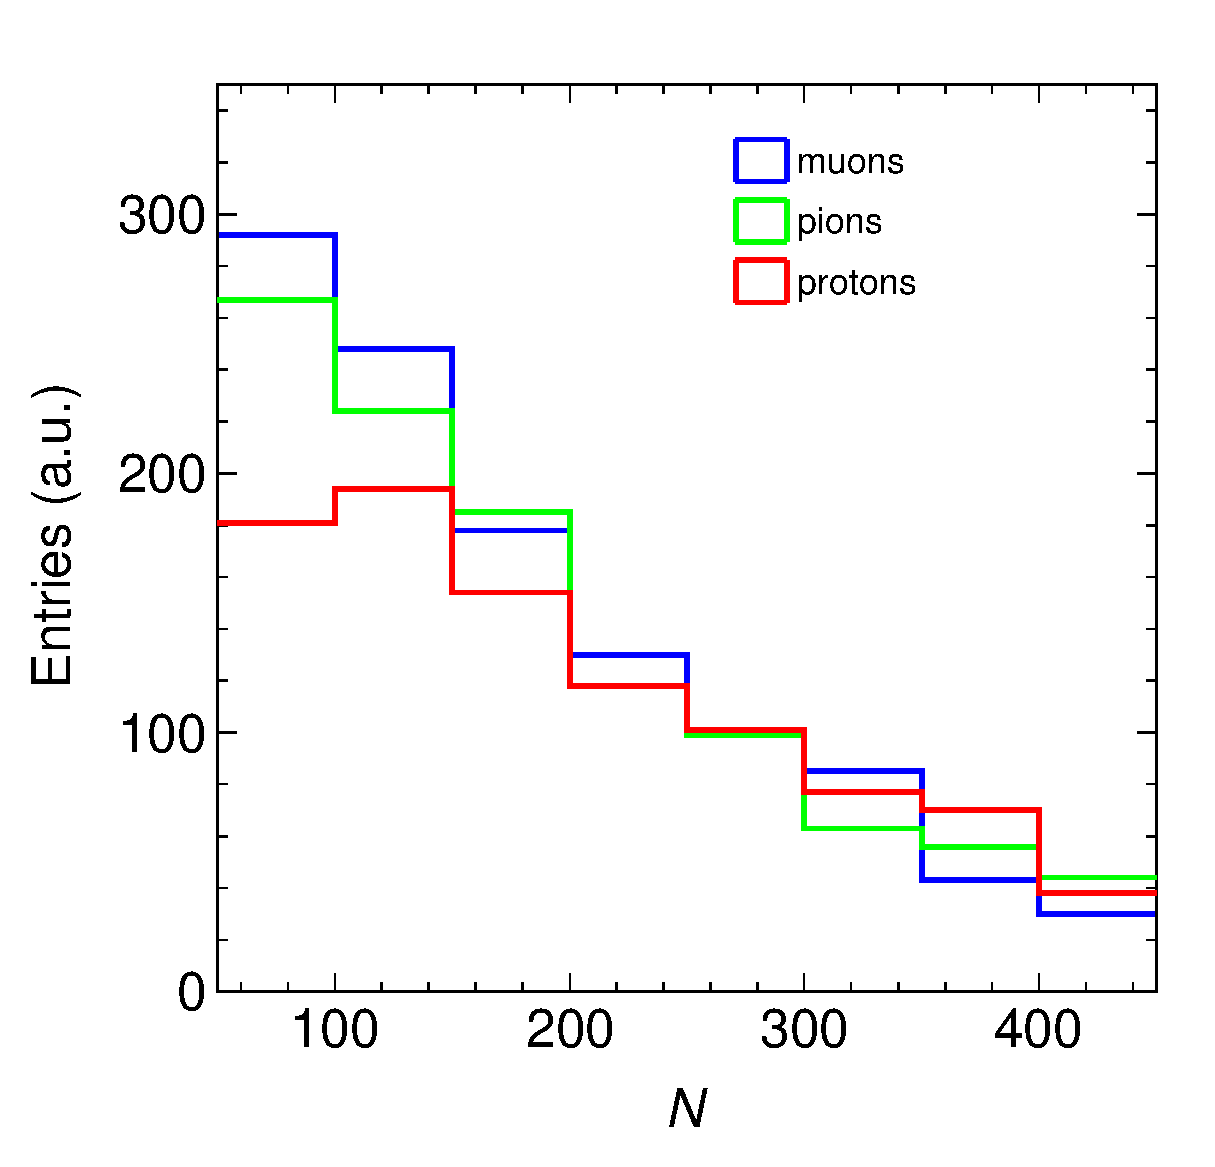
\includegraphics[width=\textwidth]{figures/ch6-TKI/Properties/ALICEStRecoGAr_Nparticles.eps}
         \caption{}
         \label{fig:ALICEStRecoGAr_Nparticles}
     \end{subfigure}
     \begin{subfigure}[b]{0.32\textwidth}
         \centering
         \includegraphics[width=\textwidth]{figures/ch6-TKI/Properties/ALICEStRecoGAr_lArmMCparticles.eps}
         \caption{}
    \label{fig:ALICEStRecoGAr_lArmMCparticles}
     \end{subfigure}
     \begin{subfigure}[b]{0.32\textwidth}
         \centering
         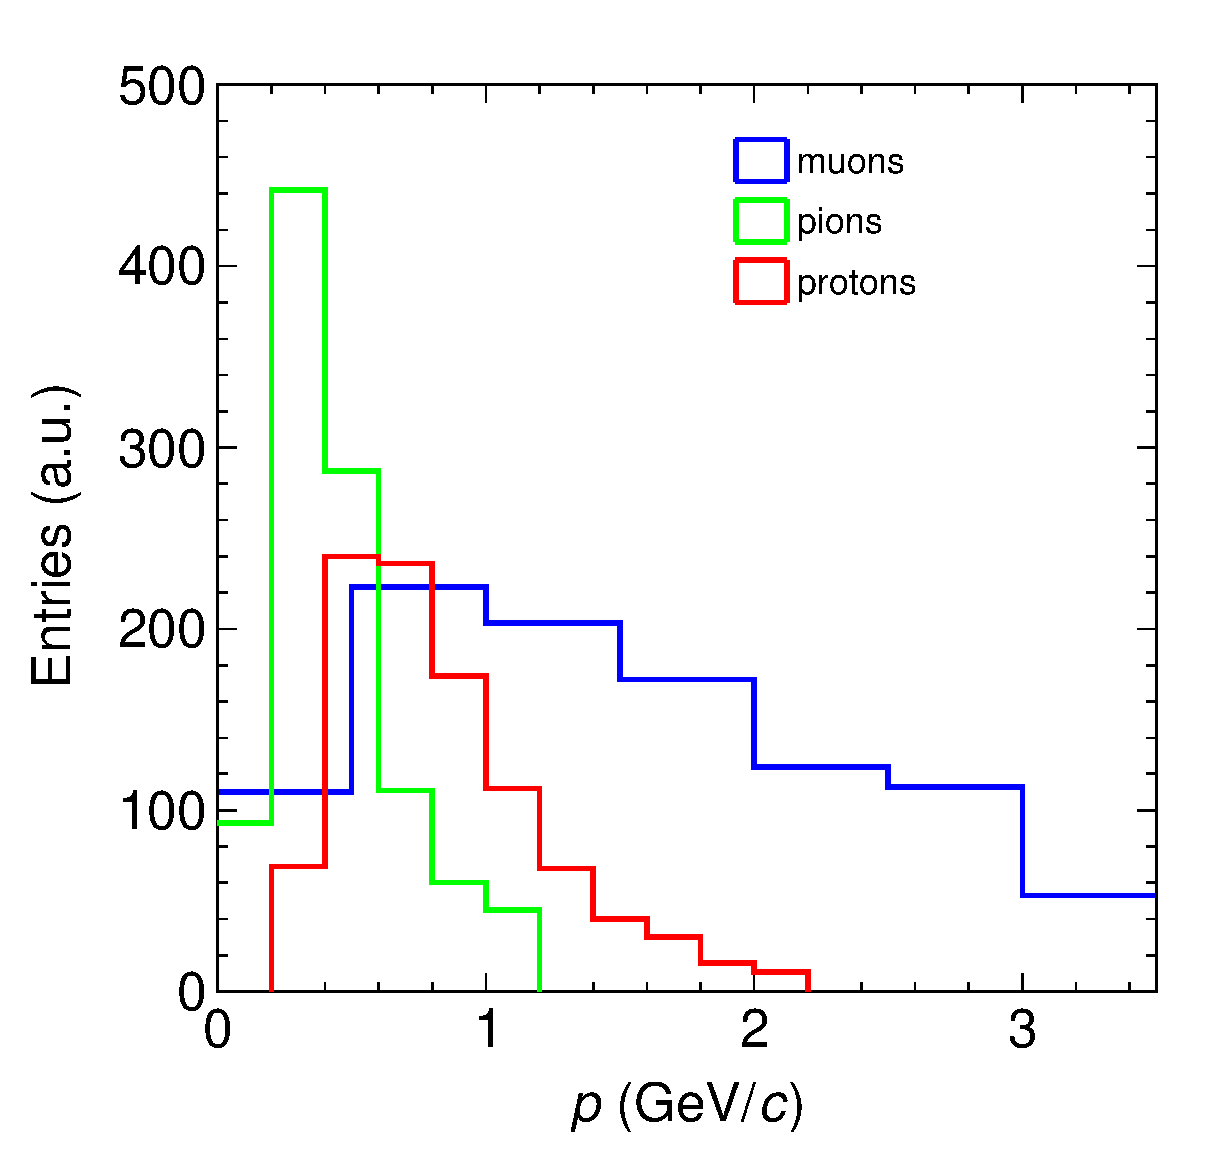
\includegraphics[width=\textwidth]{figures/ch6-TKI/Properties/ALICEStRecoGAr_pparticles.eps}
         \caption{}
         \label{fig:ALICEStRecoGAr_pparticles}
     \end{subfigure}
     \begin{subfigure}[b]{0.32\textwidth}
         \centering
         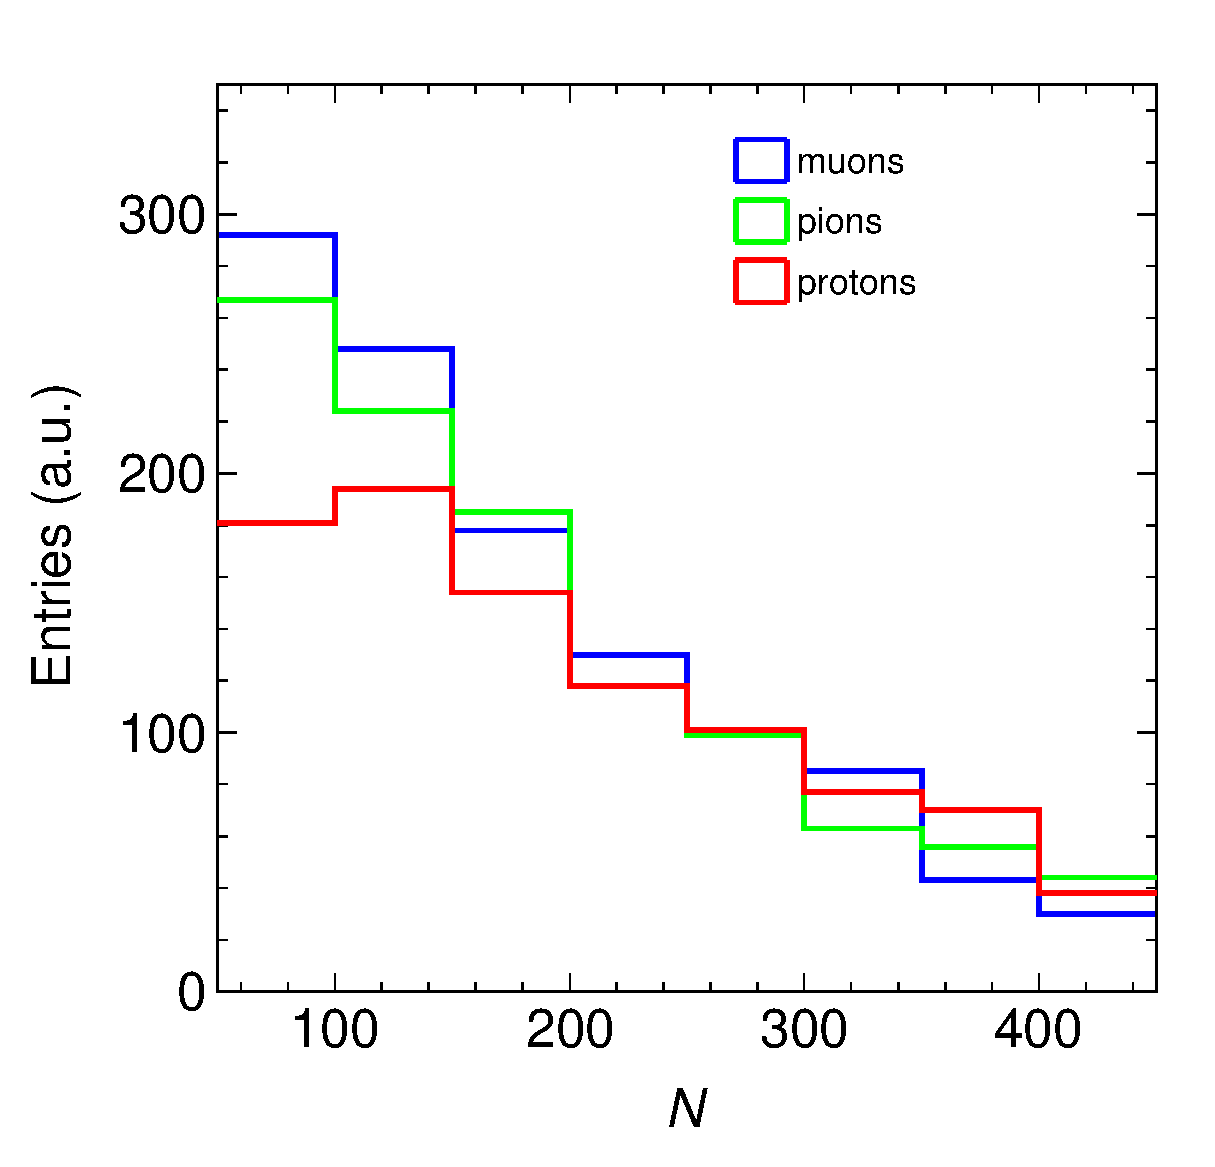
\includegraphics[width=\textwidth]{figures/ch6-TKI/Properties/ALICEStRecoGAr_Nparticles.eps}
         \caption{}
         \label{fig:GAr_Nparticles}
     \end{subfigure}
     \begin{subfigure}[b]{0.32\textwidth}
         \centering
         \includegraphics[width=\textwidth]{figures/ch6-TKI/Properties/ALICEStRecoGAr_lArmMCparticles.eps}
         \caption{}
    \label{fig:GAr_lArmMCparticles}
     \end{subfigure}
     \begin{subfigure}[b]{0.32\textwidth}
         \centering
         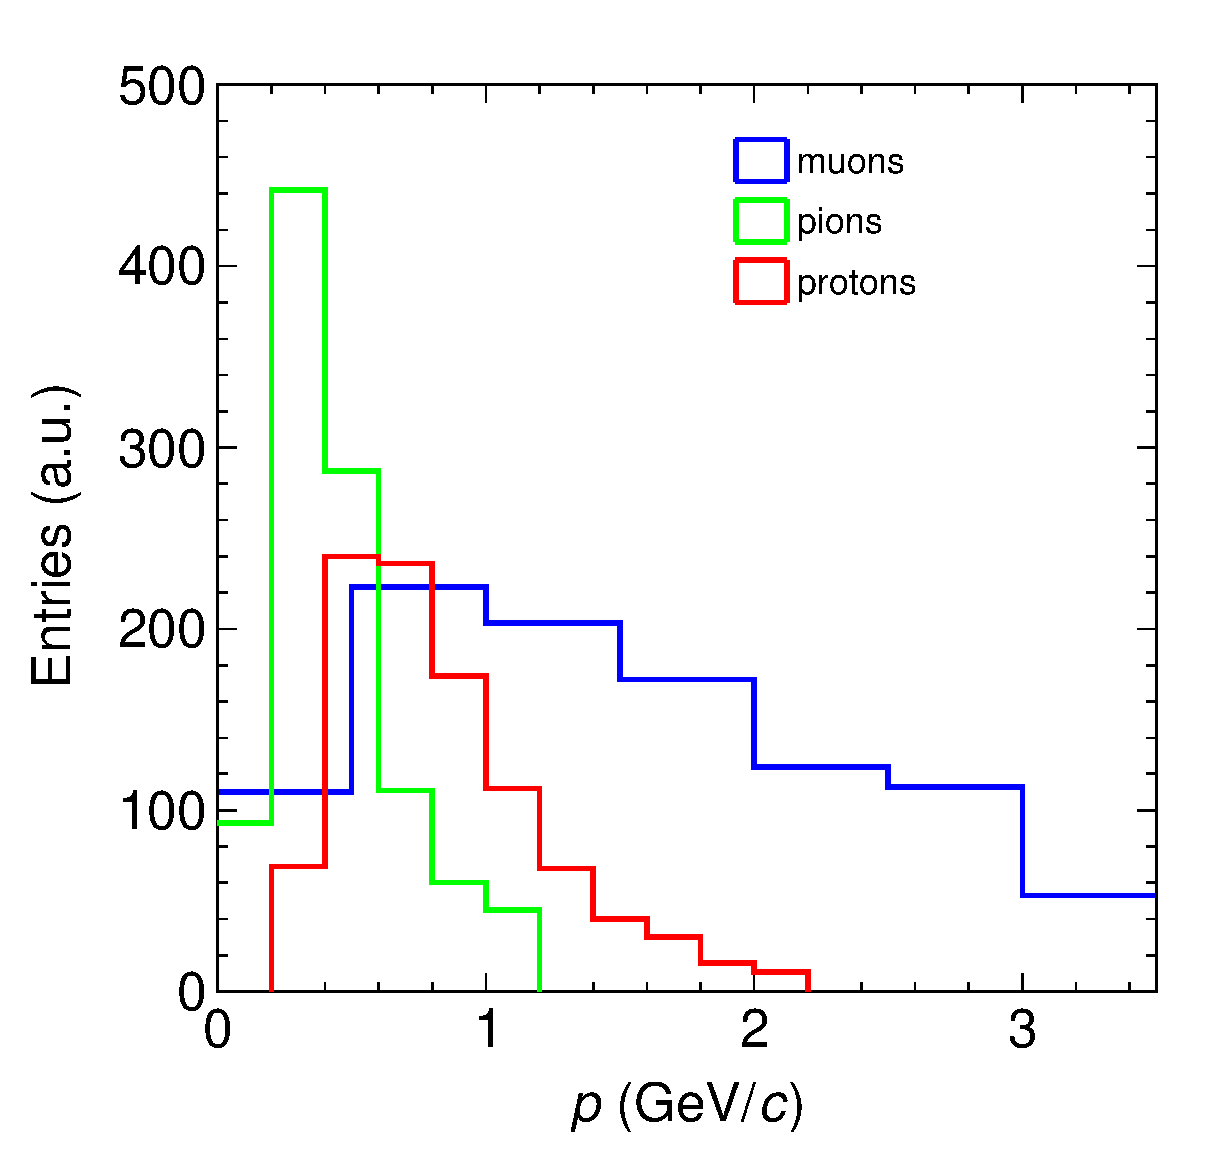
\includegraphics[width=\textwidth]{figures/ch6-TKI/Properties/ALICEStRecoGAr_pparticles.eps}
         \caption{}
         \label{fig:GAr_pparticles}
     \end{subfigure}
        \caption[Lever arm $L_\text{Arm}$, number of points $N$ and true total initial momentum $p^\text{true}$ of the particle tracks belonging to the TKI ND-GAr study.]{ Lever arm $L_\text{Arm}$, number of points $N$ and true total initial momentum $p^\text{true}$ of the particle tracks belonging to the TKI ND-GAr study. The properties for the \texttt{\texttt{CKF}} and \texttt{\texttt{GKF}} reconstructed samples are shown in the first row and second row respectively. The three charged particle types relevant for the RES interactions, which are protons, muons and pions are separated by color. } \label{fig:ALICEStRecoGAr_particles}
\end{figure}

The $\delta p_\text{TT}$ distributions divided by nuclear target are shown in Fig. \ref{fig:MC_Targets}: in the left plot the heavy nuclear target distributions are scaled to the content of the Hydrogen one, while in the right plot they are not. As expected, we see that the hydrogen distribution presents as Dirac delta peaked in 0, while the Carbon and Argon backgrounds have symmetric spreads of the order of $\mathcal{O}\sim 200 \ \text{MeV}/c$ mainly due to the isotropic smearing effect of FM as well as additional contributions from FSI. From Fig. \ref{fig:MCunscaled_Targets} we can see that using the nominal ND-GAr gas mixture, the Argon background is overwhelming, making the application of the $\delta p_\text{TT}$ technique impractical. However, as it is pointed out in Ref. \cite{Lu}, a gas TPC has the unique advantage of being able to swap the gas target with relative ease. It has been suggested that other gas mixtures with a much more favorable Argon content could be used in a HPgTPC such as ND-GAr, while still maintaining a similar detector performance and making the application of the $\delta p_\text{TT}$ technique much more realistic. As an initial proof of concept study, however, we decided to focus our attention on the nominal gas mixture. This had the obvious advantage of using the unmodified \texttt{GArSoft} simulation which has been thoroughly validated, as well as matching the conditions in which the \texttt{\texttt{CKF}} algorithm was tested and its performance evaluated.


\begin{figure}[t]
     \centering
     \begin{subfigure}[b]{0.32\textwidth}
         \centering
         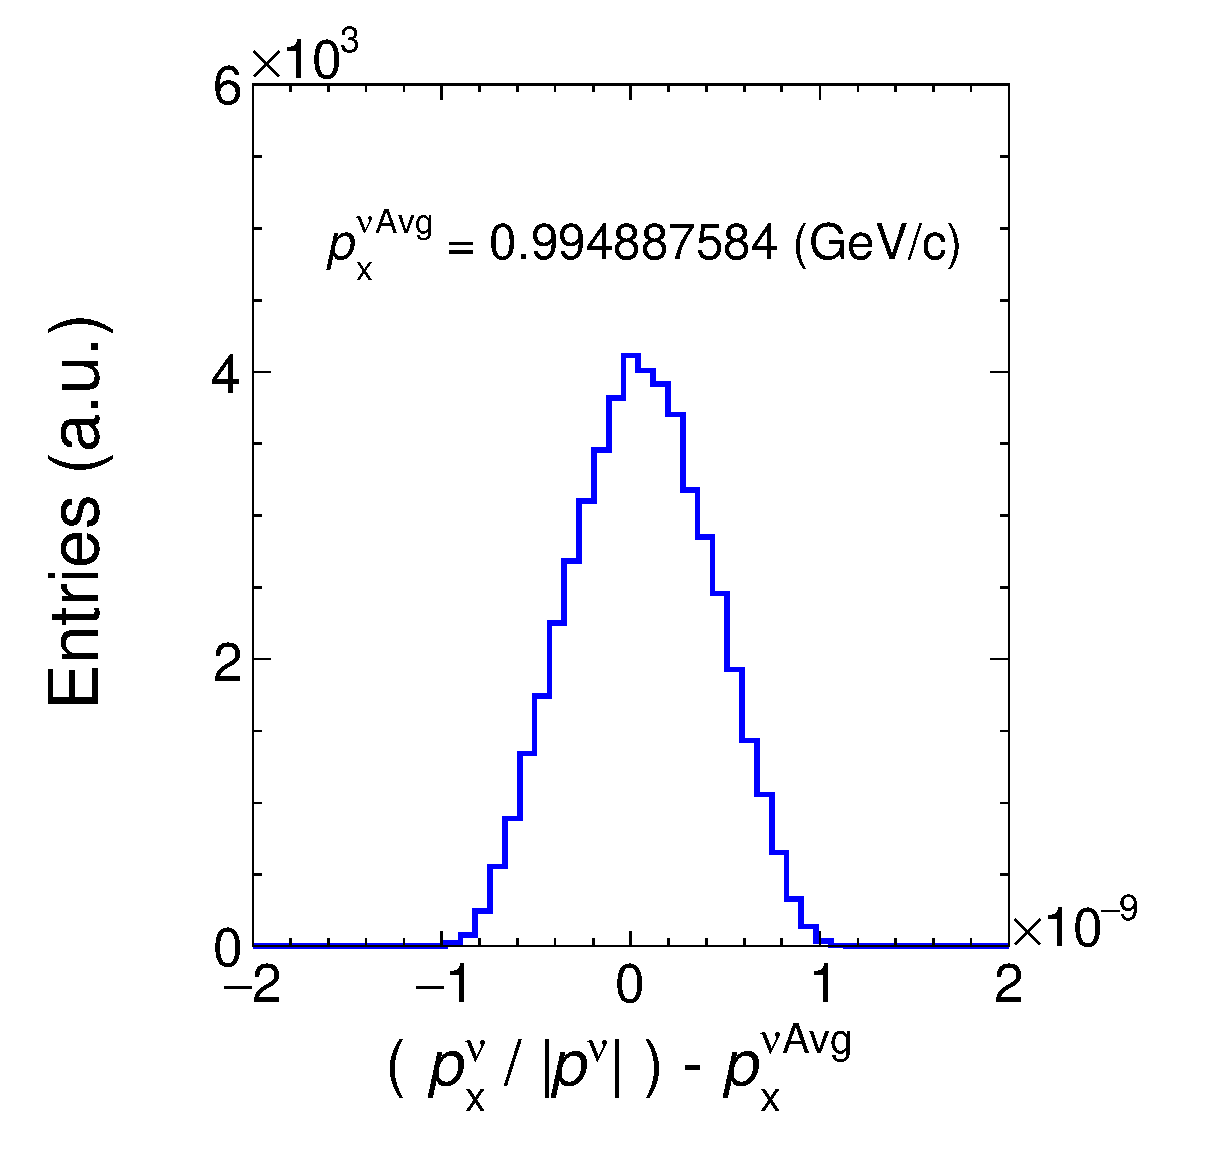
\includegraphics[width=\textwidth]{figures/ch6-TKI/Properties/NupxNorm.eps}
         \caption{}
         \label{fig:NupxNorm}
     \end{subfigure}
     \begin{subfigure}[b]{0.32\textwidth}
         \centering
         \includegraphics[width=\textwidth]{figures/ch6-TKI/Properties/NupyNorm.eps}
         \caption{}
        \label{fig:NupyNorm}
     \end{subfigure}
     \begin{subfigure}[b]{0.32\textwidth}
         \centering
         \includegraphics[width=\textwidth]{figures/ch6-TKI/Properties/NupzNorm.eps}
         \caption{}
         \label{fig:NupzNorm.eps}
     \end{subfigure}
        \caption[Distributions of the differences between the true normalized momentum components of the muon neutrinos and their average values.]{Distributions of the differences between the true normalized momentum components $p^\nu_i/|p^\nu_i|$ of the interacting muon neutrinos in the ND-GAr TKI sample and their average values $p^{\nu Avg}_i= (0.994887584,$ $ -0.100988589 , 0)$} \label{fig:NupNorm}
\end{figure}
In order to evaluate the impact of the new \texttt{CKF} reconstruction in improving the precision of the $\delta p_\text{TT}$ measurement, we applied both the \texttt{GKF} and the \texttt{CKF} reconstruction, creating two separate samples. Out of these reconstructed events, we chose those that contained exactly three tracks. This was done in order to match the topology of RES events as closely as possible, as outlined in Eq. \ref{eq:REStopology}. Additionally some quality cuts on the reconstructed properties of the tracks were applied. We selected only events for which all the tracks respected the following criteria: their reconstructed initial kinetic energy K.E. had to be 3 MeV or higher; the three momentum components $p_i$ with $i=(x,y,z)$ higher than $0.001 \ \text{GeV}/c$; the lever arm $L_\text{Arm}>50 \ \text{cm}$; the number of hit clusters belonging to the track $N>50$. The cut on the K.E. was reproduced from the original study in \cite{PhysRevC.94.015503}, while the cut on $p_i$ was made to eliminate events for which the reconstruction had failed. The two redundant cuts on the track lengths were made to eliminate the reconstructions for which the Kalman Filter technique is not suited, but for which at the moment other reconstructions are not available, as explained in Sec. \ref{sec:interactionGAr}. The $L_\text{Arm}$, $N$ and true total initial momentum $p^\text{true}$ for the particle tracks selected for the \texttt{CKF} and \texttt{GKF} reconstructed samples are shown in Fig. \ref{fig:ALICEStRecoGAr_particles} in the first and second row respectively. The three charged particle types relevant for the RES interactions, which are protons, muons and pions are separated by color. All the selected particles show to have produced similarly long tracks, while having significantly different momentum distributions. As expected from resonant events, the charged leptons $\mu^-$ has on average the highest momenta, the pions the lowest and the protons are in between.  

\begin{figure}[t]
     \centering
     \begin{subfigure}[b]{0.48\textwidth}
         \centering
         \includegraphics[width=\textwidth]{figures/ch6-TKI/1D/GAr_dpTT_numuCC_Fit.png}
         \caption{}
         \label{fig:dpTT_GArReco}
     \end{subfigure}
     \begin{subfigure}[b]{0.48\textwidth}
         \centering
         \includegraphics[width=\textwidth]{figures/ch6-TKI/1D/ALICE_dpTT_numuCC_Fit.png}
         \caption{}
         \label{fig:dpTT_ALICEReco}
     \end{subfigure}
        \caption{$\delta p_\text{TT}$ distributions for a sample of $\nu_\mu$ CC interactions in ND-GAr's TPC, calculated using reconstructed momentum quantities taken at the start of the reconstructed tracks. The different atomic targets (H,C and Ar) are separated by color. The \texttt{GKF} and \texttt{CKF} reconstructions have been used in the left (a) and right (b) plot respectively. The results of a Cauchy fit applied to the Hydrogen distributions are shown directly on the plots.} \label{fig:dpTT}
\end{figure}

The reconstructed neutrino direction was taken as the average values of the true normalized momentum components $p^\nu_i/|p^\nu_i|$ which were: $p^{\nu Avg}_i = (0.994887584,$ $ -0.100988589 , 0) \ \text{GeV}/c$. The distributions of the differences between $p^\nu_i/|p^\nu_i|$ and $p^{\nu Avg}_i$ are shown on Fig. \ref{fig:NupNorm}. As can be seen from the spread of the distributions, which are of the order of $10^{-6} \ \text{GeV}/c$ for the $x$ and $y$ components and $10^{-16} \ \text{GeV}/c$ for the $z$ components, no significant smearing was applied to the neutrino flux during the GENIE interaction simulation phase. This makes the impact of the uncertainty on the neutrino direction in this study negligible. 

The Hydrogen target $\delta p_\text{TT}$ distributions obtained using the \texttt{CKF} and \texttt{GKF} reconstruction are shown in Fig. \ref{fig:dpTT}. The Argon and Carbon distributions are also shown, scaled to the content of the Hydrogen one. In both cases the reconstructed momentum was taken at the start of the track, rather than at the interaction vertex, as it was done for the MC results. The Hydrogen distributions were fitted with a Cauchy probability density function as defined in Eq. \ref{eq:Cauchy}. For the \texttt{GKF} the distribution is unbiased, having $m=(-0.3\pm1.0) \ \text{MeV}/c$ and has a spread of $\sigma = 19.7\pm1.3 \ \text{MeV}/c$, which is comparable with the results obtained for the T2K ND280 detector. Better results are obtained with the \texttt{CKF} algorithm, for which we obtain an unbiased $m=(1.2\pm0.7) \ \text{MeV}/c$ but a $\sigma = 14.8\pm0.9 \ \text{MeV}/c$, showing an improvement which is compatible with the momentum reconstruction performance demonstrated for the algorithm in Sec. \ref{sec:interactionGAr}.

\begin{figure}[t]
         \centering
         \includegraphics[width=0.58\textwidth]{figures/ch6-TKI/1D/MC_dpTT_numuCC_Fit.png}
        \caption{$\delta p_\text{TT}$ distributions for a sample of $\nu_\mu$ CC interactions in ND-GAr's TPC, calculated using true momentum quantities taken at the start of the reconstructed tracks. The different atomic targets (H,C and Ar) are separated by color. The results of a Cauchy fit applied to the Hydrogen distributions are shown directly on the plots. } \label{fig:dpTTMC_TrackStart}
\end{figure}

Additional performance improvements can be obtained by propagating the reconstruction of the 3 tracks to the interaction vertex. This can be easily done with a Kalman Filter by simply adding the interaction vertex as an additional point to the start of each track. In order to gauge how much resolution is lost exclusively by the misplacement of the track starting point, we can calculate the $\delta p_\text{TT}$ spread using the true momentum components associated with the closest trajectory points to the the starting hit clusters of each track. We show the distribution resulting from this calculation in Fig. \ref{fig:dpTTMC_TrackStart}. We again fitted the distribution using a Cauchy p.d.f. obtaining a spread of $\sigma = (3.6\pm0.2) \ \text{MeV}/c$. This implies that if the propagation to the interaction vertex is done perfectly, the resolution can be improved by up to $\sim 3.6 \ \text{MeV}/c$. 

\begin{figure}[t]
     \centering
     \begin{subfigure}[b]{0.48\textwidth}
         \centering
         \includegraphics[width=\textwidth]{figures/ch6-TKI/1D/ALICEStMC_dpTT_numuCC_Fit.png}
         \caption{}
         \label{fig:dpTT_ALICEStMCReco}
     \end{subfigure}
    \begin{subfigure}[b]{0.48\textwidth}
         \centering
         \includegraphics[width=\textwidth]{figures/ch6-TKI/1D/ALICEStRecoGAr_dpTT_numuCC_Fit.png}
         \caption{}  \label{fig:dpTT_ALICEStRecoGArReco}
     \end{subfigure}
        \caption{$\delta p_\text{TT}$ distributions for a sample of $\nu_\mu$ CC interactions in ND-GAr's TPC, calculated using reconstructed momentum quantities propagated to the true (a) and reconstructed (b) interaction vertex. In both cases the \texttt{CKF} has been used for the reconstruction. The results of a Cauchy fit applied to the Hydrogen distributions are shown directly on the plots. } \label{fig:dpTTVertex}
\end{figure}

\begin{figure}[t]
     \centering
     \begin{subfigure}{0.32\textwidth}
         \centering
         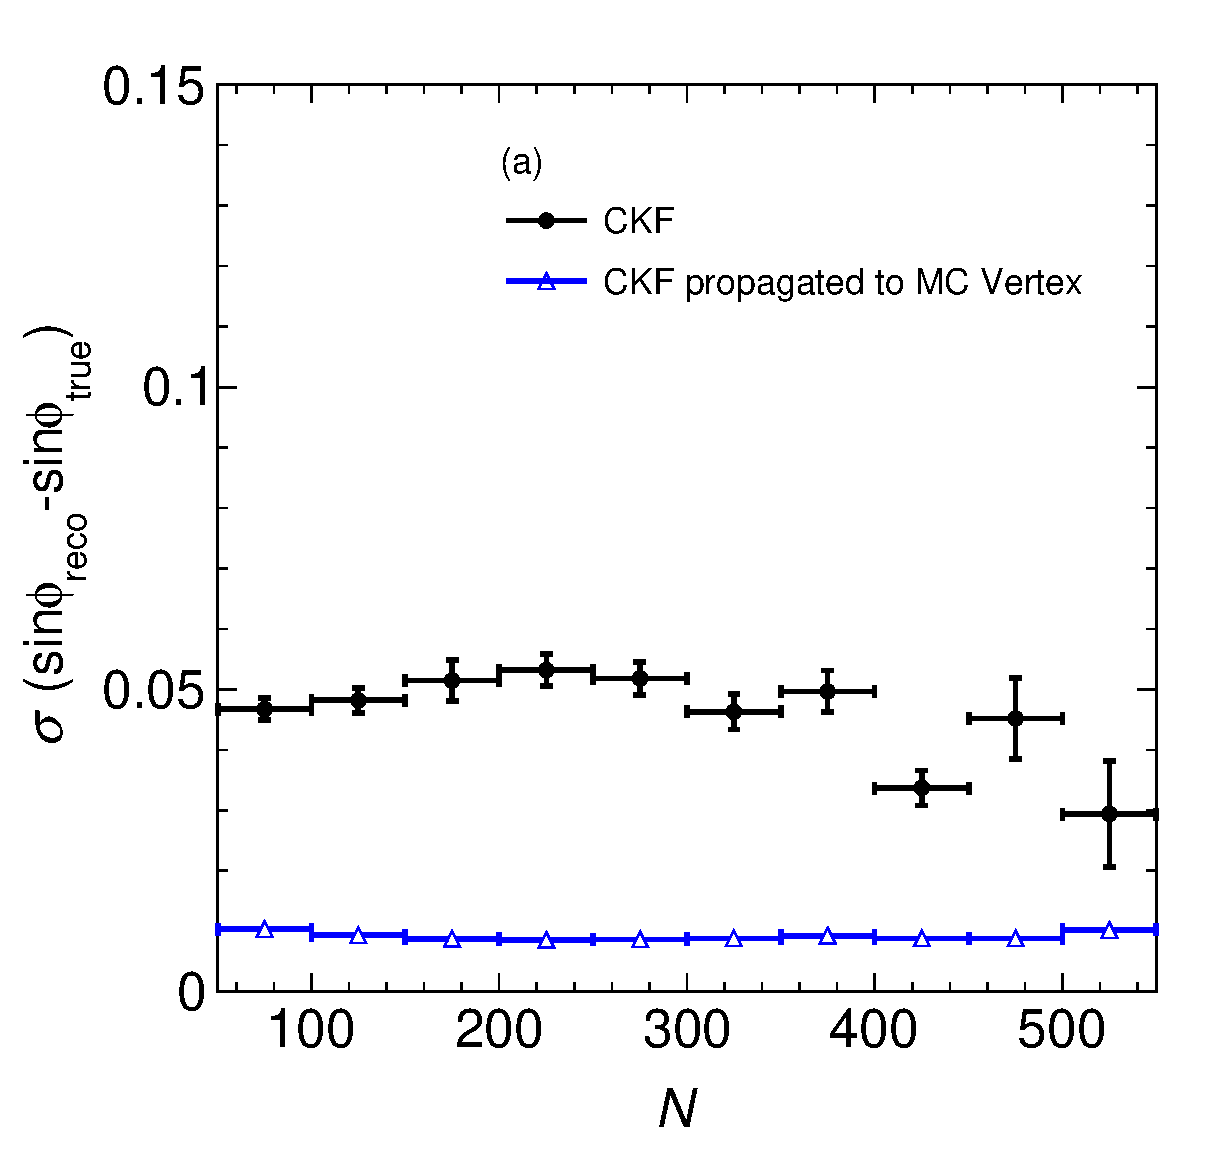
\includegraphics[width=\textwidth]{figures/ch6-TKI/sinphiRes/RessinphiVSNPoints_VertexComparison_13.eps}
         \caption{} \label{fig:RessinphiVSNPoints_VertexComparison_13}
     \end{subfigure}
     \begin{subfigure}{0.32\textwidth}
         \centering
        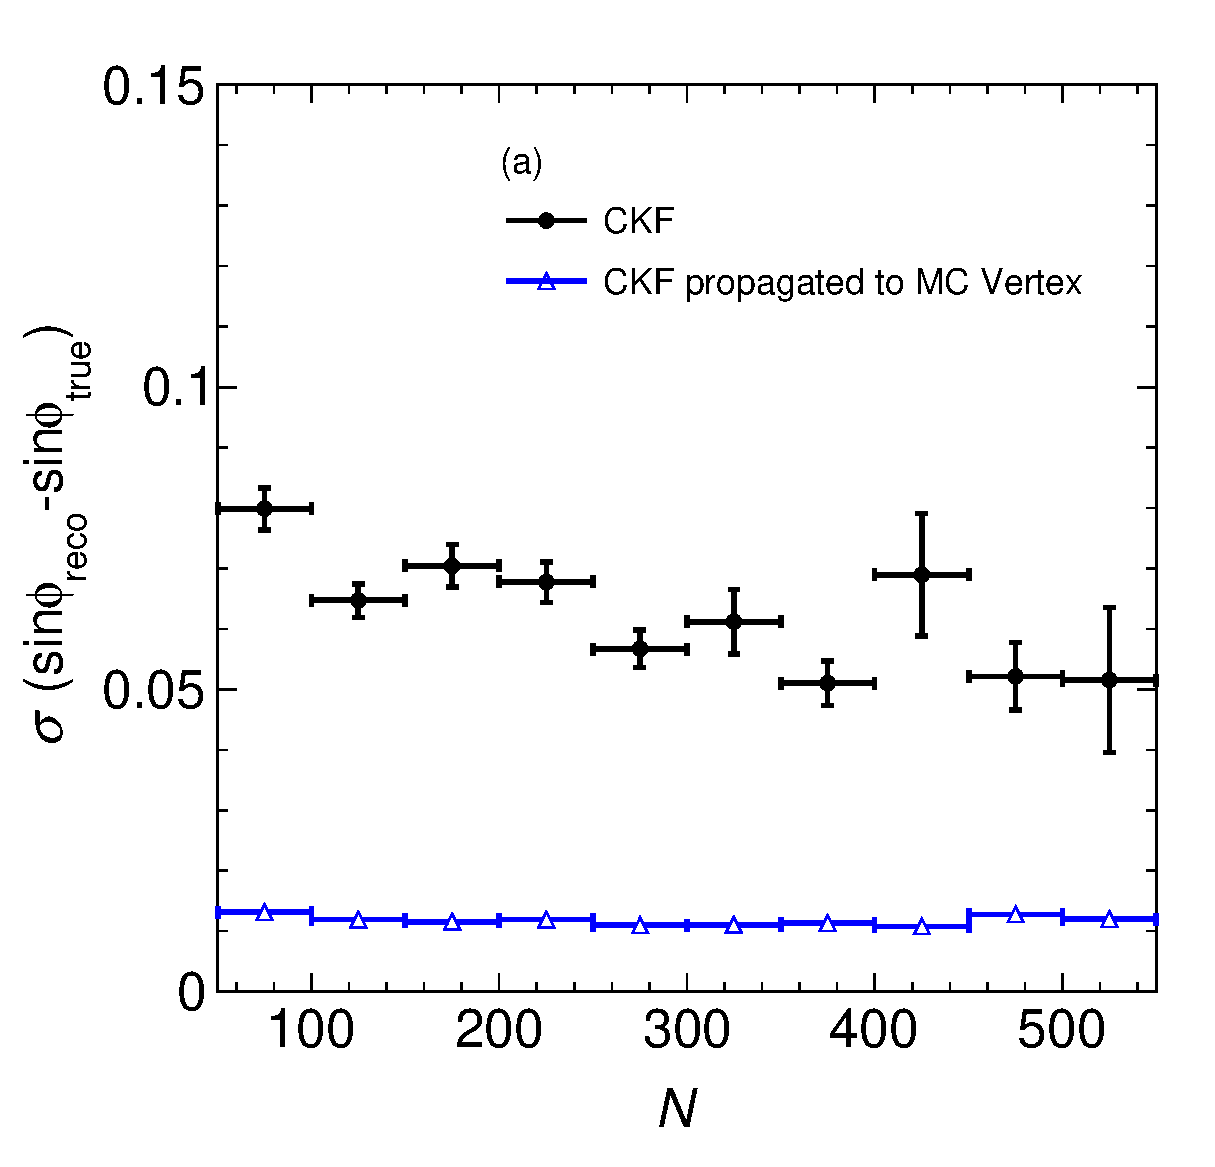
\includegraphics[width=\textwidth]{figures/ch6-TKI/sinphiRes/RessinphiVSNPoints_VertexComparison_211.eps}
         \caption{} \label{fig:RessinphiVSNPoints_VertexComparison_211}
     \end{subfigure}
    \begin{subfigure}{0.32\textwidth}
         \centering
        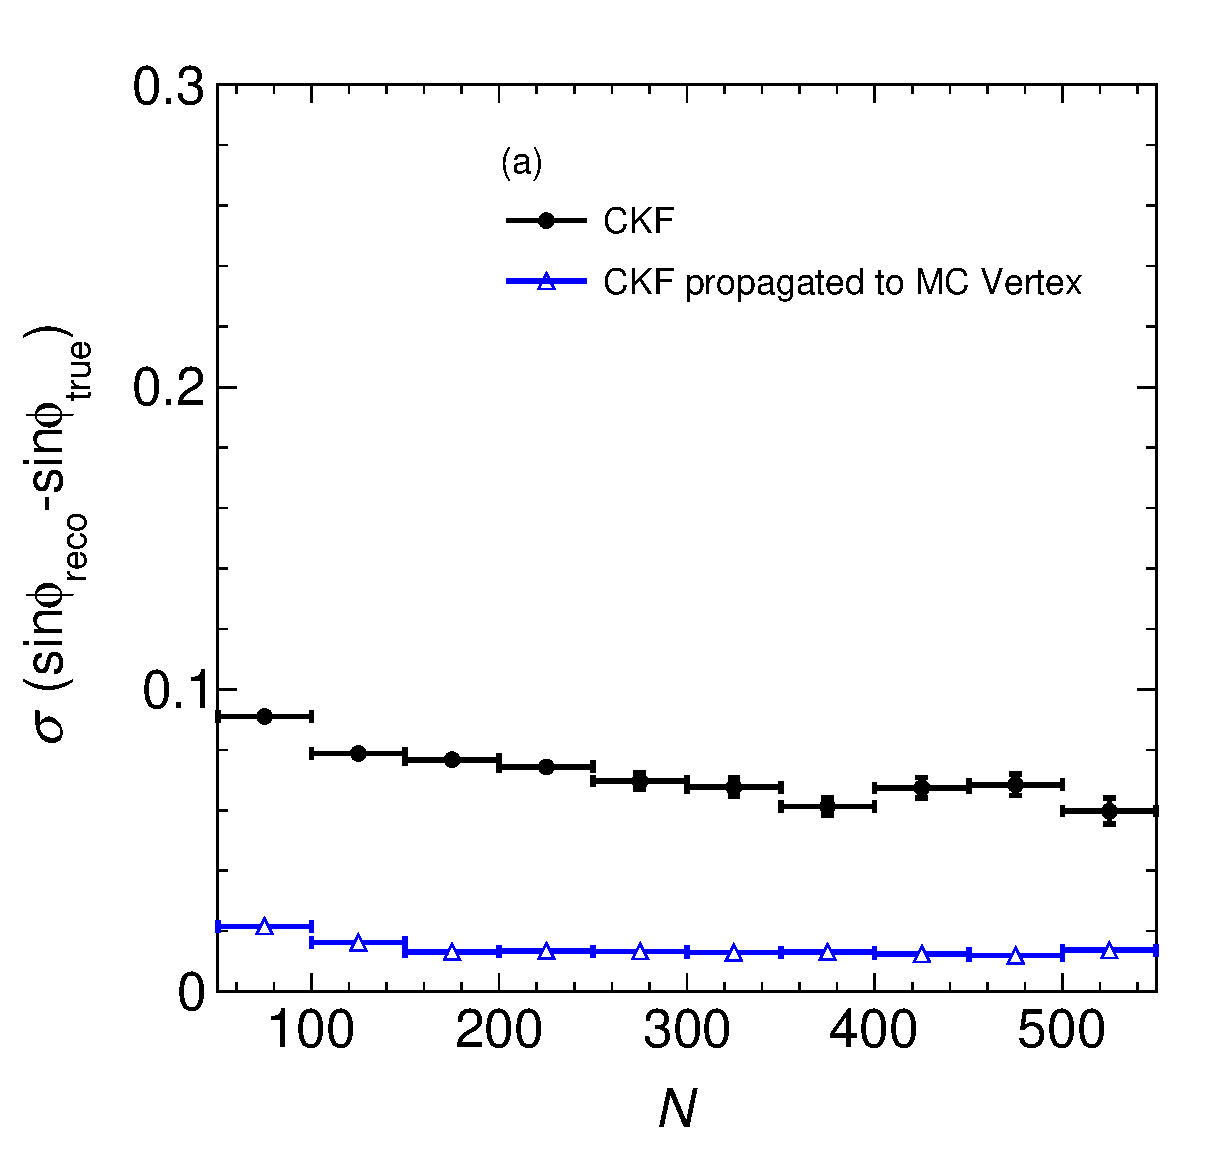
\includegraphics[width=\textwidth]{figures/ch6-TKI/sinphiRes/RessinphiVSNPoints_VertexComparison_2212.eps}
         \caption{} \label{fig:RessinphiVSNPoints_VertexComparison_2212}
     \end{subfigure}
          \begin{subfigure}{0.32\textwidth}
         \centering
        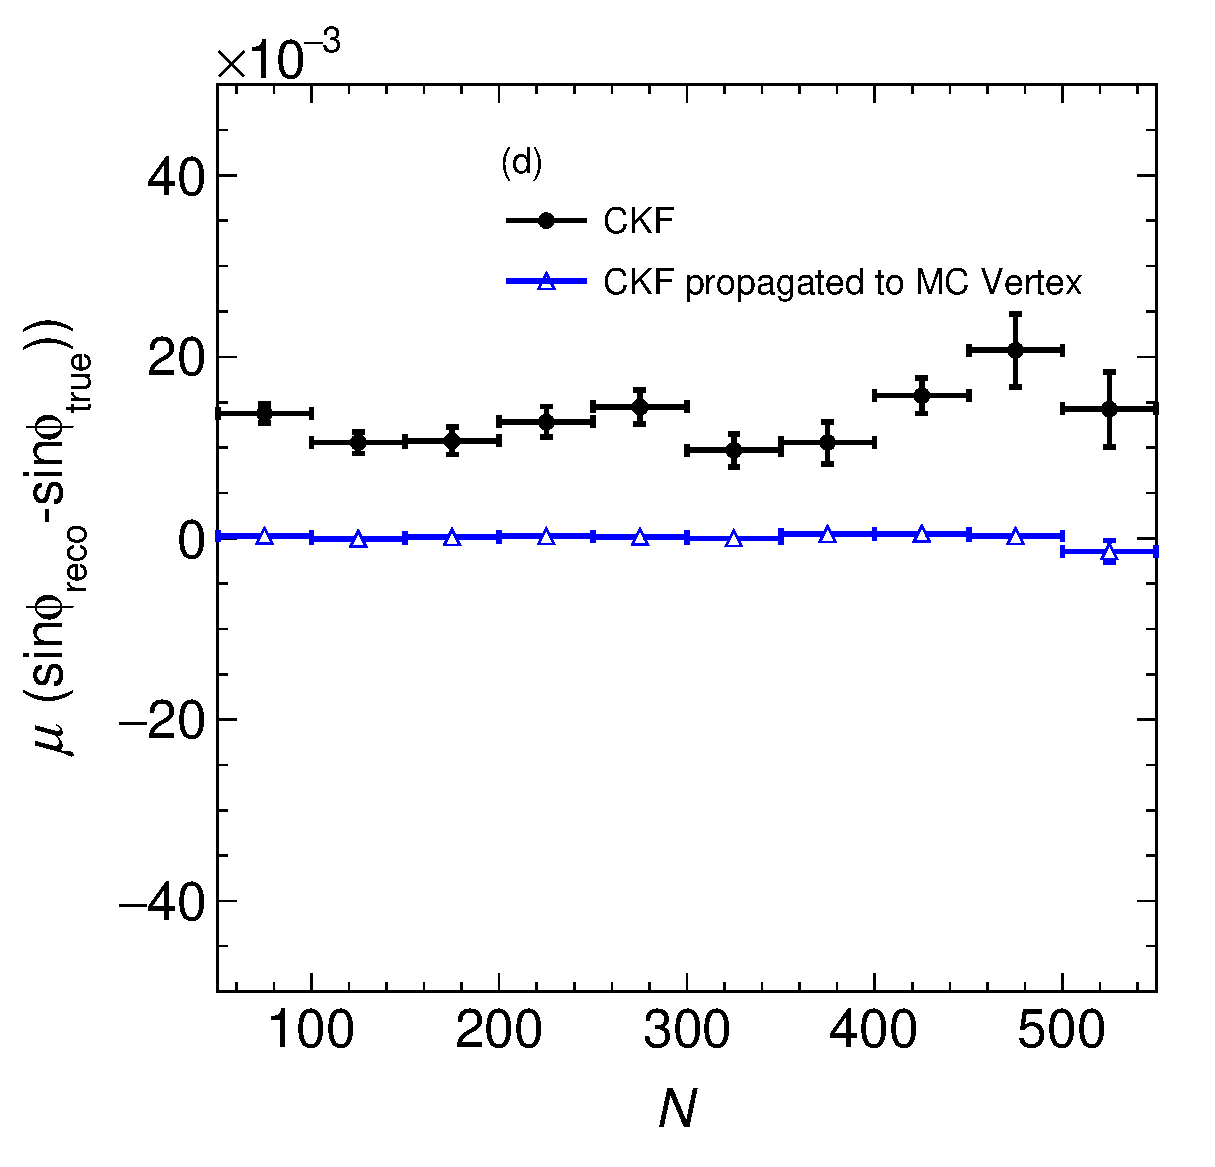
\includegraphics[width=\textwidth]{figures/ch6-TKI/sinphiRes/BiassinphiVSNPoints_VertexComparison_13.eps}
         \caption{} \label{fig:BiassinphiVSNPoints_VertexComparison_13}
     \end{subfigure}
     \begin{subfigure}{0.32\textwidth}
         \centering
        \includegraphics[width=\textwidth]{figures/ch6-TKI/sinphiRes/BiassinphiVSNPoints_VertexComparison_211.eps}
         \caption{} \label{fig:BiassinphiVSNPoints_VertexComparison_211}
     \end{subfigure}
          \begin{subfigure}{0.32\textwidth}
         \centering
        \includegraphics[width=\textwidth]{figures/ch6-TKI/sinphiRes/BiassinphiVSNPoints_VertexComparison_2212.eps}
         \caption{} \label{fig:BiassinphiVSNPoints_VertexComparison_2212}
     \end{subfigure}
        \caption{Resolution and bias of the $\sin\phi$ parameter in the hydrogen $\nu_\mu$ CC ND-GAr sample, as a function of the number of points in the tracks $N$. In black we show the results obtained with the \texttt{CKF} before the propagation, and in blue we show them after. The results for the three different particle types are shown from left to right in increasing order of mass (i.e. $\mu^-$, $\pi^+$ and $p$) with the resolution on top ((a),(b) and (c)) and the bias at the bottom ((a),(b) and (c)).  The bias and resolution are defined as the $\mu$ and $\sigma$ of simple Gaussian fits applied to the $\sin\phi$ residuals. The residuals are taken in comparison to the $\sin\phi$ true values at the interaction vertex.}
        \label{fig:sinphiRes2DNPoints_Vertex}
\end{figure}


We applied the propagation to the \texttt{CKF} algorithm, using both the true coordinates of the interaction vertex, as well as the reconstructed ones from \texttt{GArSoft}. The results are shown in Figs. \ref{fig:dpTT_ALICEStMCReco} and \ref{fig:dpTT_ALICEStRecoGArReco} respectively. When using the true position of the vertex, the \texttt{CKF} is capable of fully recovering the $3.6 \ \text{MeV}/c$ smearing, reaching a Cauchy spread of $\sigma= (11.3\pm0.7) \ \text{MeV}/c$. If the reconstructed vertex is used instead, the smearing is still mostly corrected for, reaching a Cauchy spread of $\sigma= (11.9\pm0.7) \ \text{MeV}/c$. This result is compatible with our original expectations derived from the momentum reconstruction performance of the \texttt{CKF}.

\begin{figure}[t]
     \centering
     \begin{subfigure}[b]{0.32\textwidth}
         \centering
         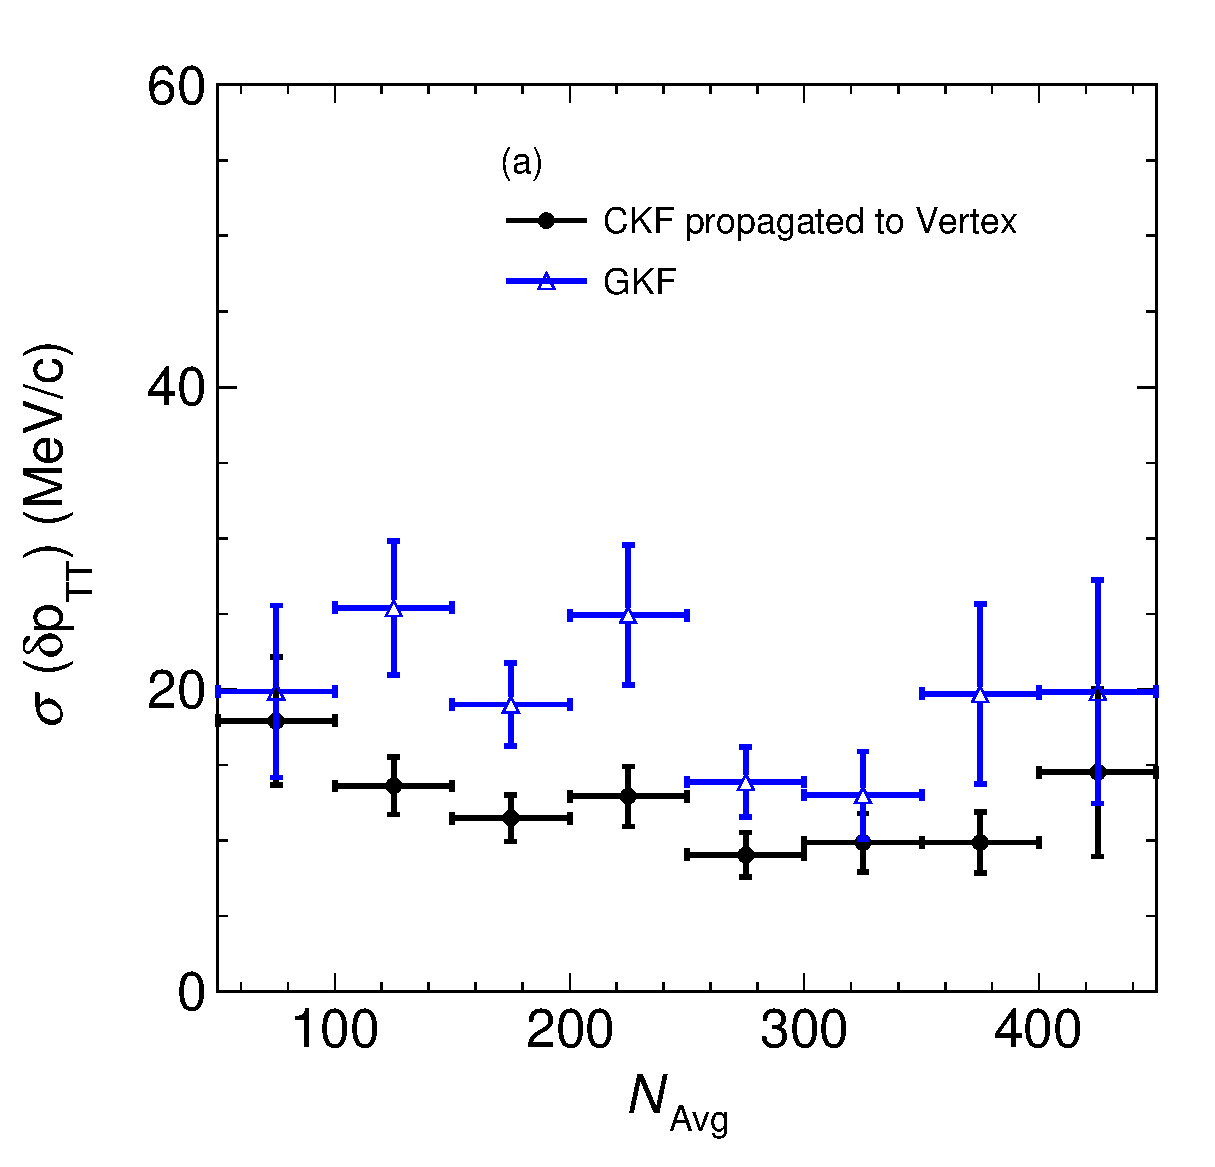
\includegraphics[width=\textwidth]{figures/ch6-TKI/2D/deltapTTVSAvgN.eps}
         \caption{}
         \label{fig:deltapTTVSAvgN}
     \end{subfigure}
     \begin{subfigure}[b]{0.32\textwidth}
         \centering
         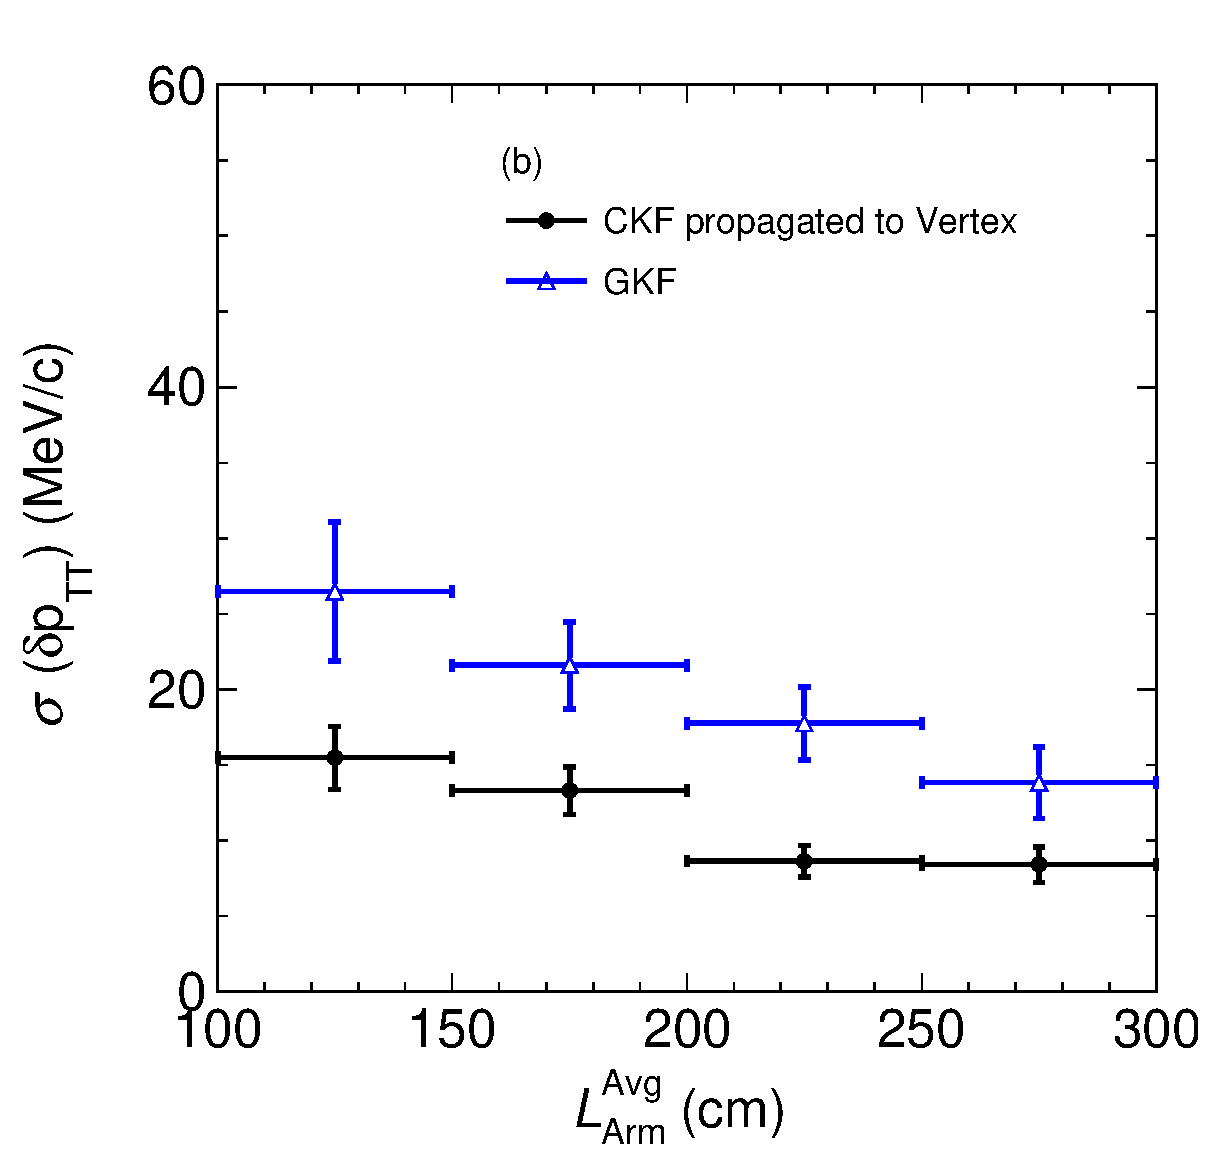
\includegraphics[width=\textwidth]{figures/ch6-TKI/2D/deltapTTVSAvglArmMC.eps}
         \caption{}
        \label{fig:deltapTTVSAvglArmMC.eps}
     \end{subfigure}
     \begin{subfigure}[b]{0.32\textwidth}
         \centering
         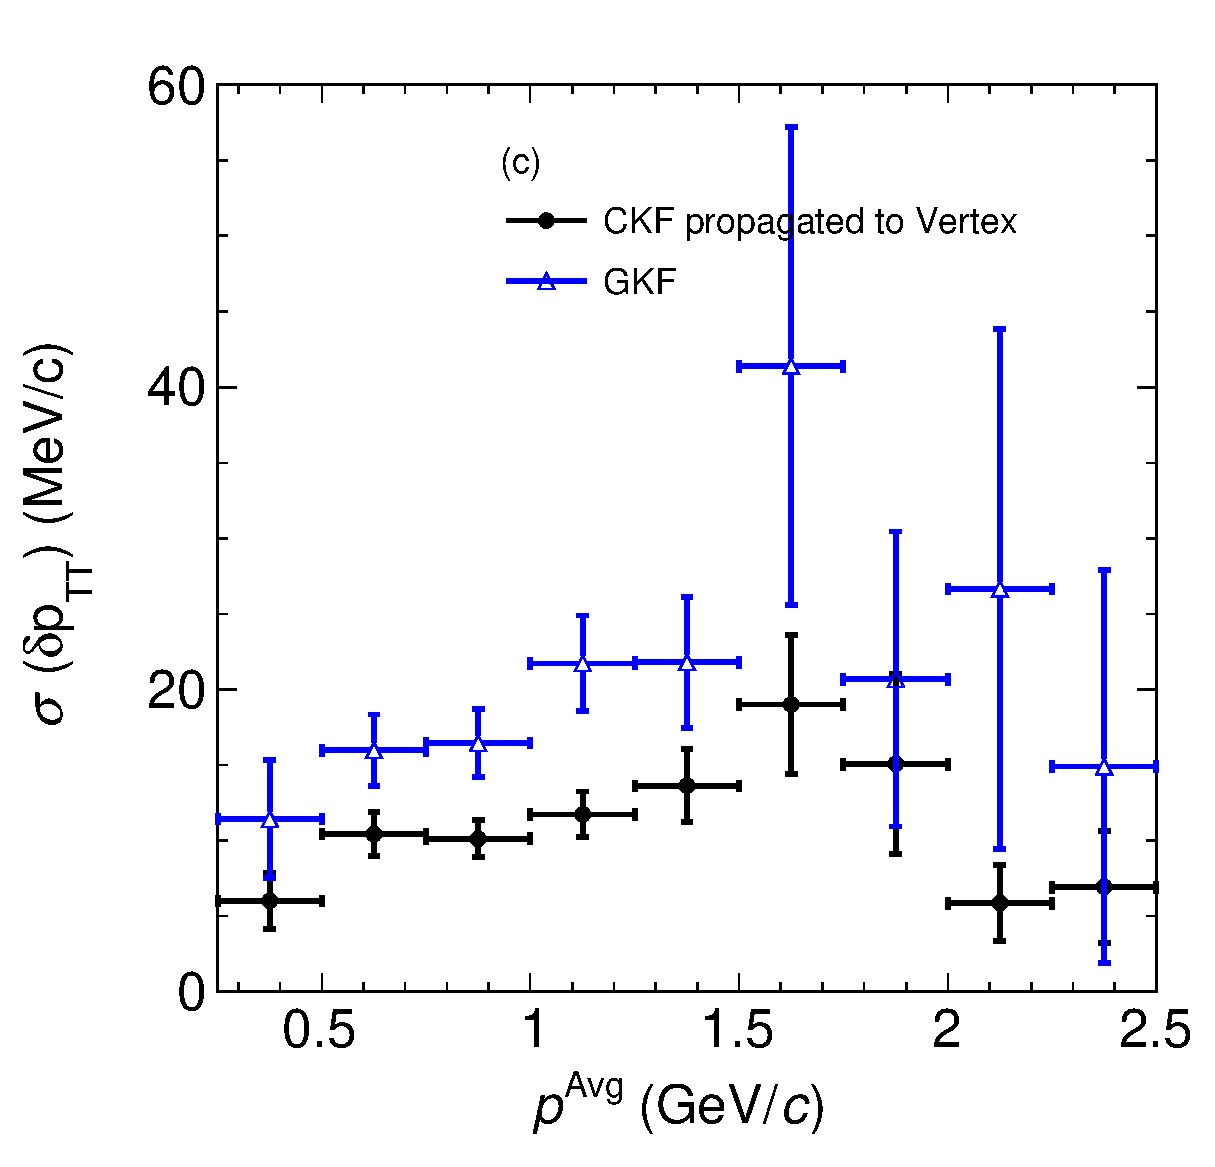
\includegraphics[width=\textwidth]{figures/ch6-TKI/2D/deltapTTVSAvgp.eps}
         \caption{}
         \label{fig:deltapTTVSAvgp.eps}
     \end{subfigure}
        \caption{Dependency of the $\delta p_\texttt{TT}$ Cauchy spread Hydrogen resolution as a function of average number of points $N$, lever arm $L_\text{Arm}$ and true initial momentum $p$, calculated between the three tracks in the event. In blue we show the results obtained with the \texttt{\texttt{GKF}}, while in black we show the results for the \texttt{\texttt{CKF}} propagated to the reconstructed vertex.} \label{fig:dpTTVSAvg}
\end{figure}

The improvement in resolution obtained after the vertex propagation of the \texttt{CKF} can mostly be attributed to a better estimation of the momentum angles at the interaction point. To illustrate this in Fig. \ref{fig:sinphiRes2DNPoints_Vertex} we show the resolution and bias of the $\sin\phi$ parameter in the Hydrogen sample, as a function of the number of points in the tracks. In black we show the results obtained with the \texttt{CKF} before the propagation, and in blue we show them after. The results for the three different particle types are shown from left to right in increasing order of mass (i.e. $\mu^-$, $\pi^+$ and $p$) .  As done previously the bias and resolution are defined as the $\mu$ and $\sigma$ of simple Gaussian fits applied to the $\sin\phi$ residuals. In this case the residuals are taken in comparison to the $\sin\phi$ true values at the interaction vertex. Note that this is different from what was done previously, where the closest trajectory point was always considered. For all particle types, both the resolution and bias are significantly improved. It is interesting to note that the direction of the $\sin\phi$ bias is opposite for particles of opposite charge: negative for the $p$ and $\pi^+$ and positive for the $\mu^-$. This is consistent with the opposite direction of circular motion that we expect for particles of opposite charge in a magnetic field.

In Figs. \ref{fig:dpTTVSAvg} and \ref{fig:dpTTVSpart} we show the dependency of the $\delta p_\texttt{TT}$ resolution as a function of number of points $N$, lever arm $L_\text{Arm}$ and true initial momentum $p$. In Fig.\ref{fig:dpTTVSAvg} we show the dependency on the average values calculated among the three tracks in each event, while in \ref{fig:dpTTVSpart} we show the dependency on the characteristics of each particle type. In all cases the resolution is defined again as the Cauchy spread of the $\delta p_\text{TT}$ Hydrogen distribution. In blue we show the results obtained with the \texttt{\texttt{GKF}}, while in black we show the results for the \texttt{\texttt{CKF}} propagated to the reconstructed vertex. It is clear that the \texttt{\texttt{CKF}} outperforms the old algorithm , regardless of the tracks characteristics. Since the $\delta p_\text{TT}$ resolution on Hydrogen solely depends on the detector response, we should expect for the dependencies to follow similar patterns to the ones described by the Gluckstern formulas in Eqs. \ref{eq:sigmaNptot} and \ref{eq:sigmaMSptot}. Indeed, looking at the dependencies on the average properties of the tracks, we see an inverse proportionality on $L_\text{Arm}$ and $N$ and a direct proportionality on $p$, which is in agreement with expectations. The dependencies are less clear but still visible when looking at the particle types separately.

\begin{figure}[t]
     \centering
     \begin{subfigure}[b]{0.32\textwidth}
         \centering
         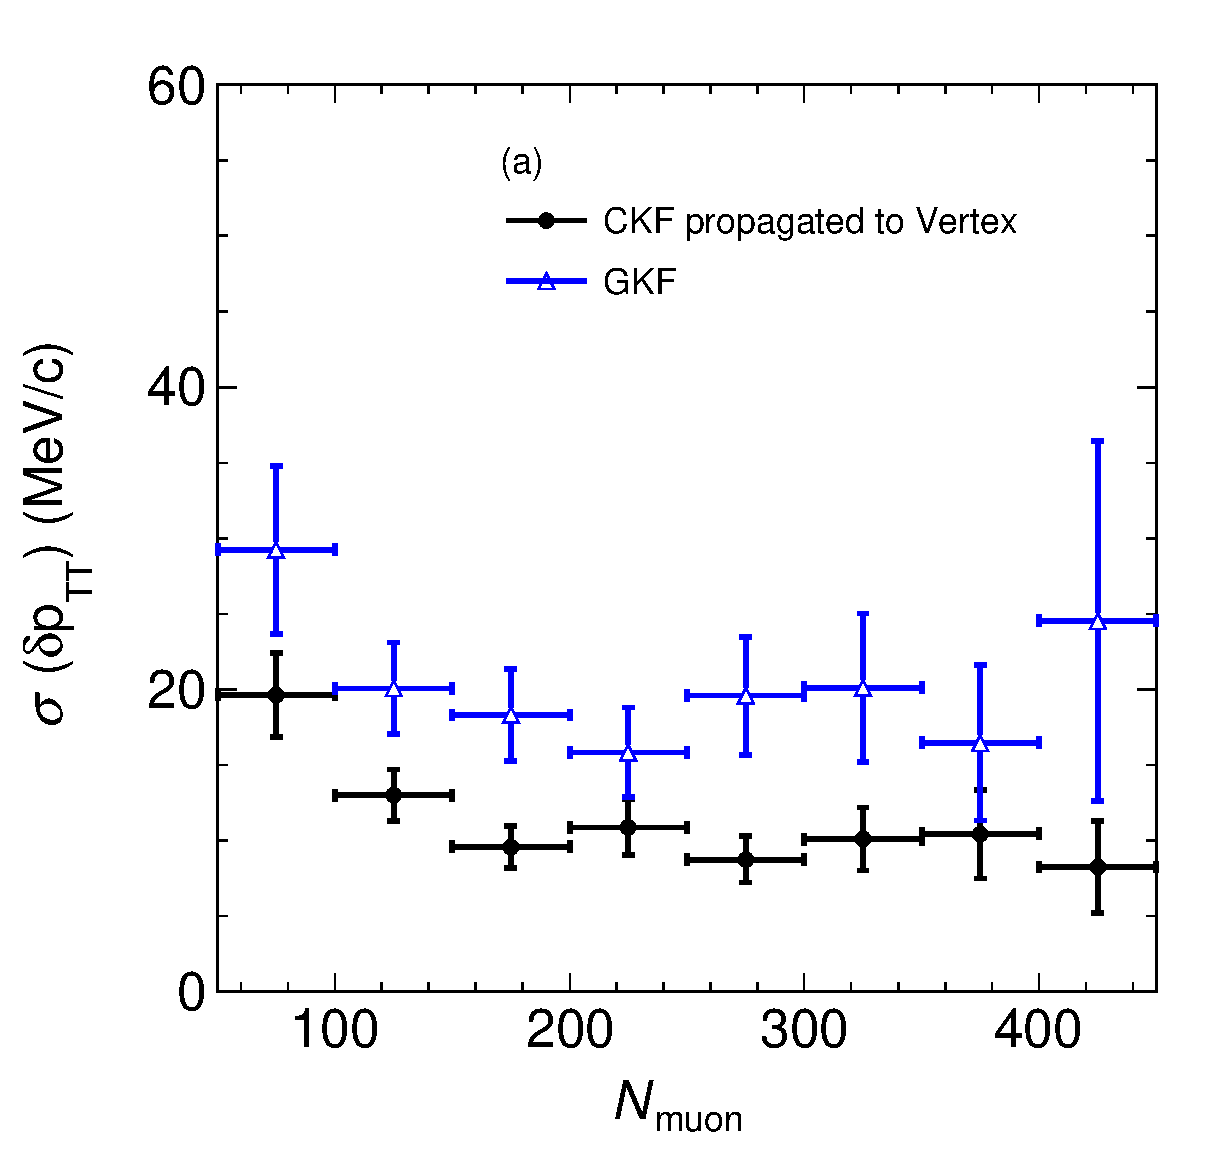
\includegraphics[width=\textwidth]{figures/ch6-TKI/2D/deltapTTVSN13.eps}
         \caption{}
         \label{fig:deltapTTVSN13}
     \end{subfigure}
     \begin{subfigure}[b]{0.32\textwidth}
         \centering
         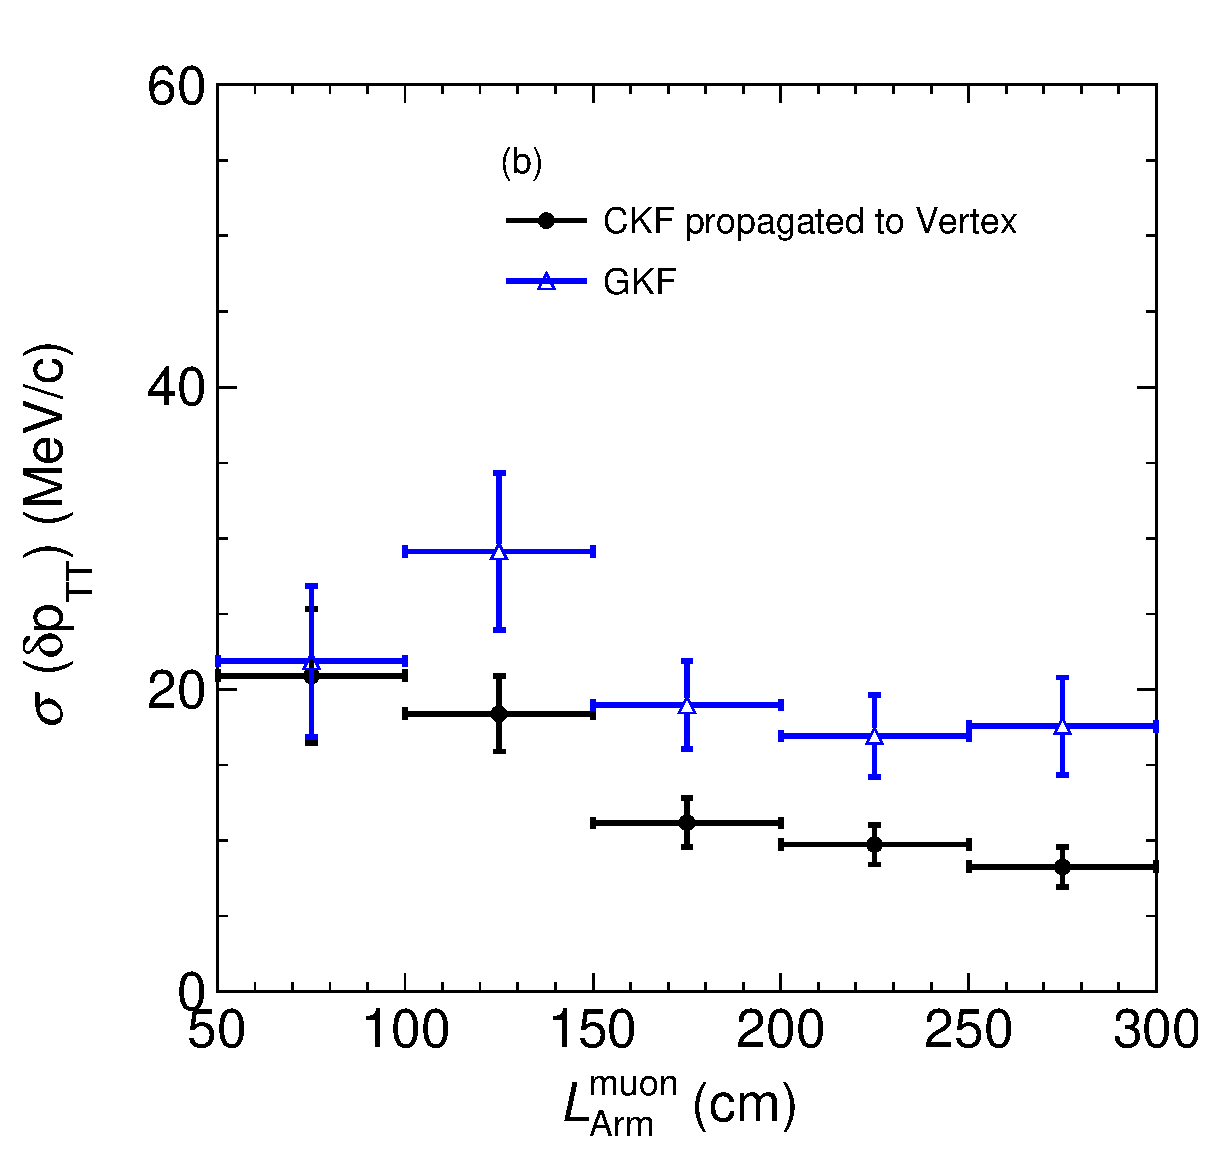
\includegraphics[width=\textwidth]{figures/ch6-TKI/2D/deltapTTVSlArmMC13.eps}
         \caption{}
        \label{fig:deltapTTVSlArmMC13.eps}
     \end{subfigure}
     \begin{subfigure}[b]{0.32\textwidth}
         \centering
         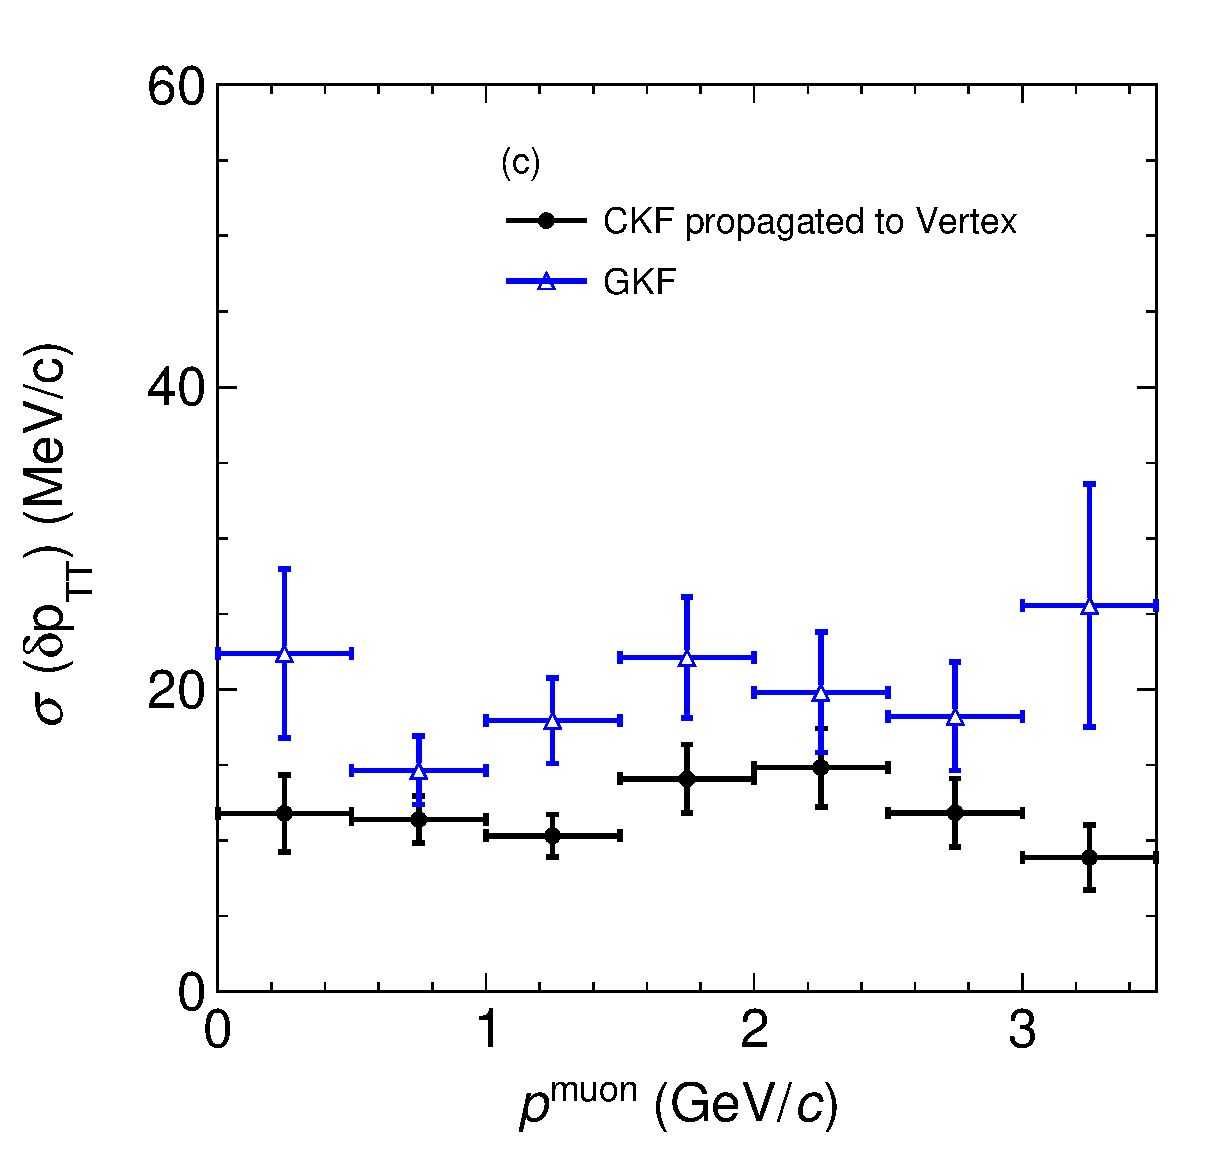
\includegraphics[width=\textwidth]{figures/ch6-TKI/2D/deltapTTVSp13.eps}
         \caption{}
         \label{fig:deltapTTVSp13.eps}
     \end{subfigure}
     
          \begin{subfigure}[b]{0.32\textwidth}
         \centering
         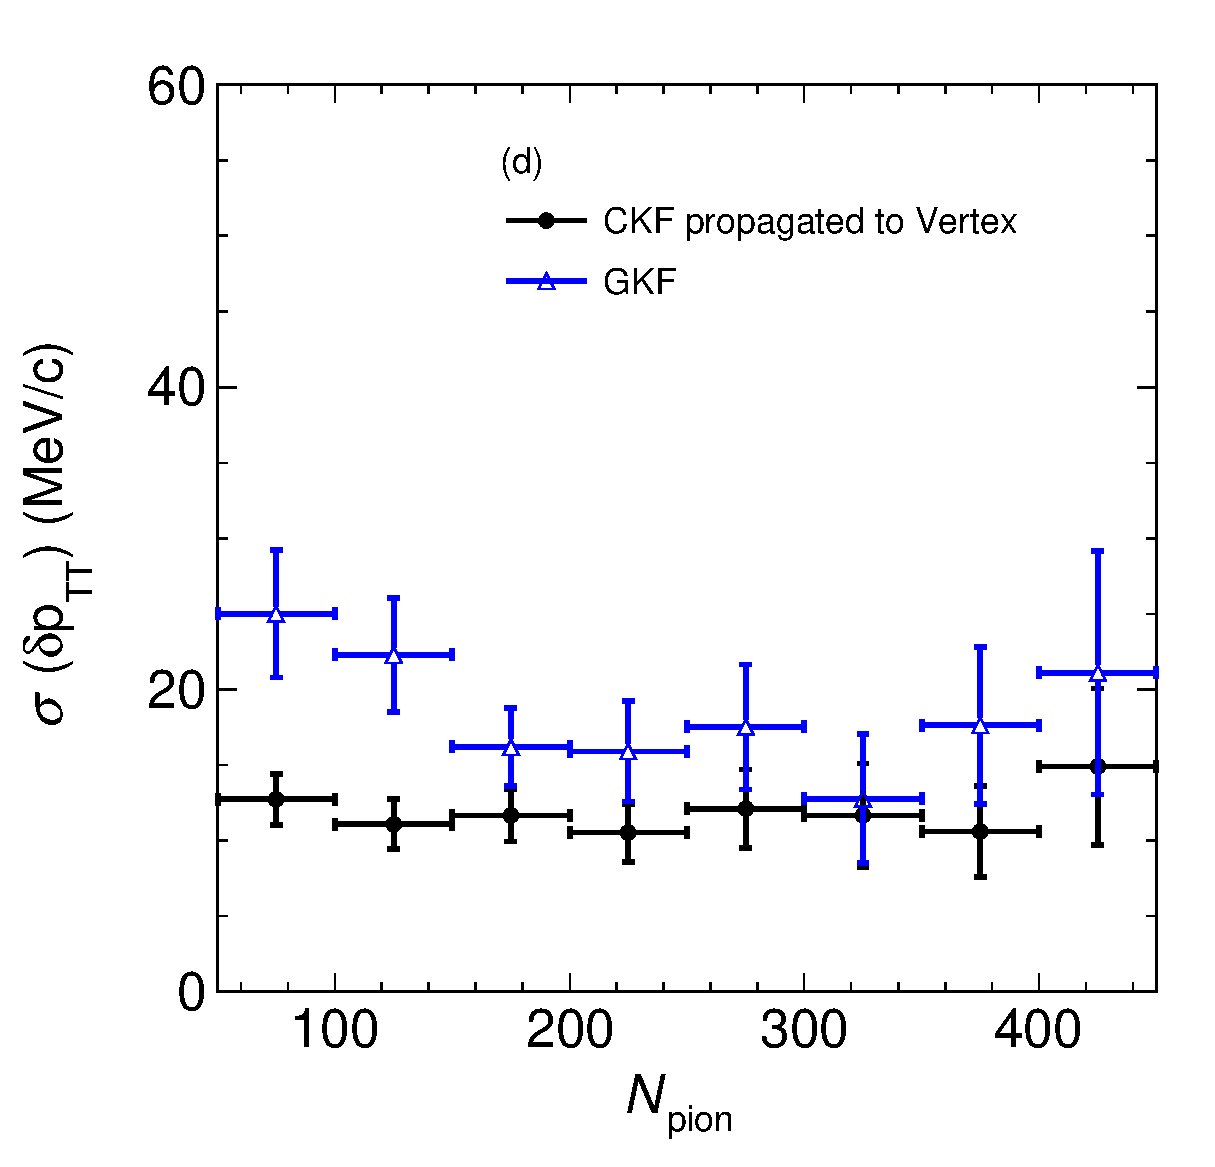
\includegraphics[width=\textwidth]{figures/ch6-TKI/2D/deltapTTVSN211.eps}
         \caption{}
         \label{fig:deltapTTVSN211}
     \end{subfigure}
     \begin{subfigure}[b]{0.32\textwidth}
         \centering
         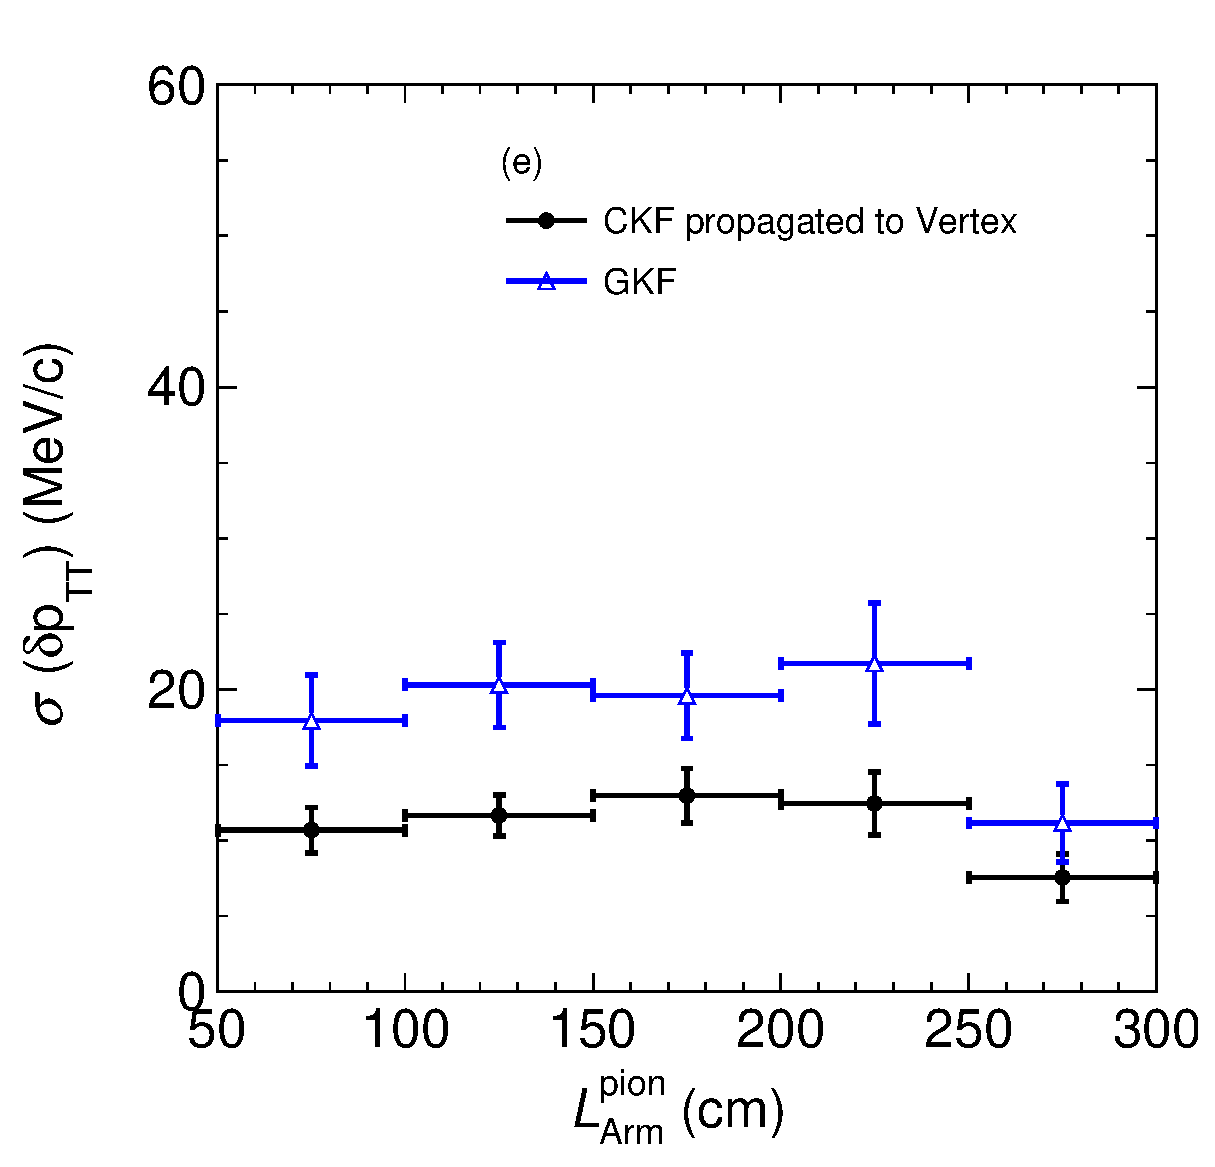
\includegraphics[width=\textwidth]{figures/ch6-TKI/2D/deltapTTVSlArmMC211.eps}
         \caption{}
        \label{fig:deltapTTVSlArmMC211.eps}
     \end{subfigure}
     \begin{subfigure}[b]{0.32\textwidth}
         \centering
         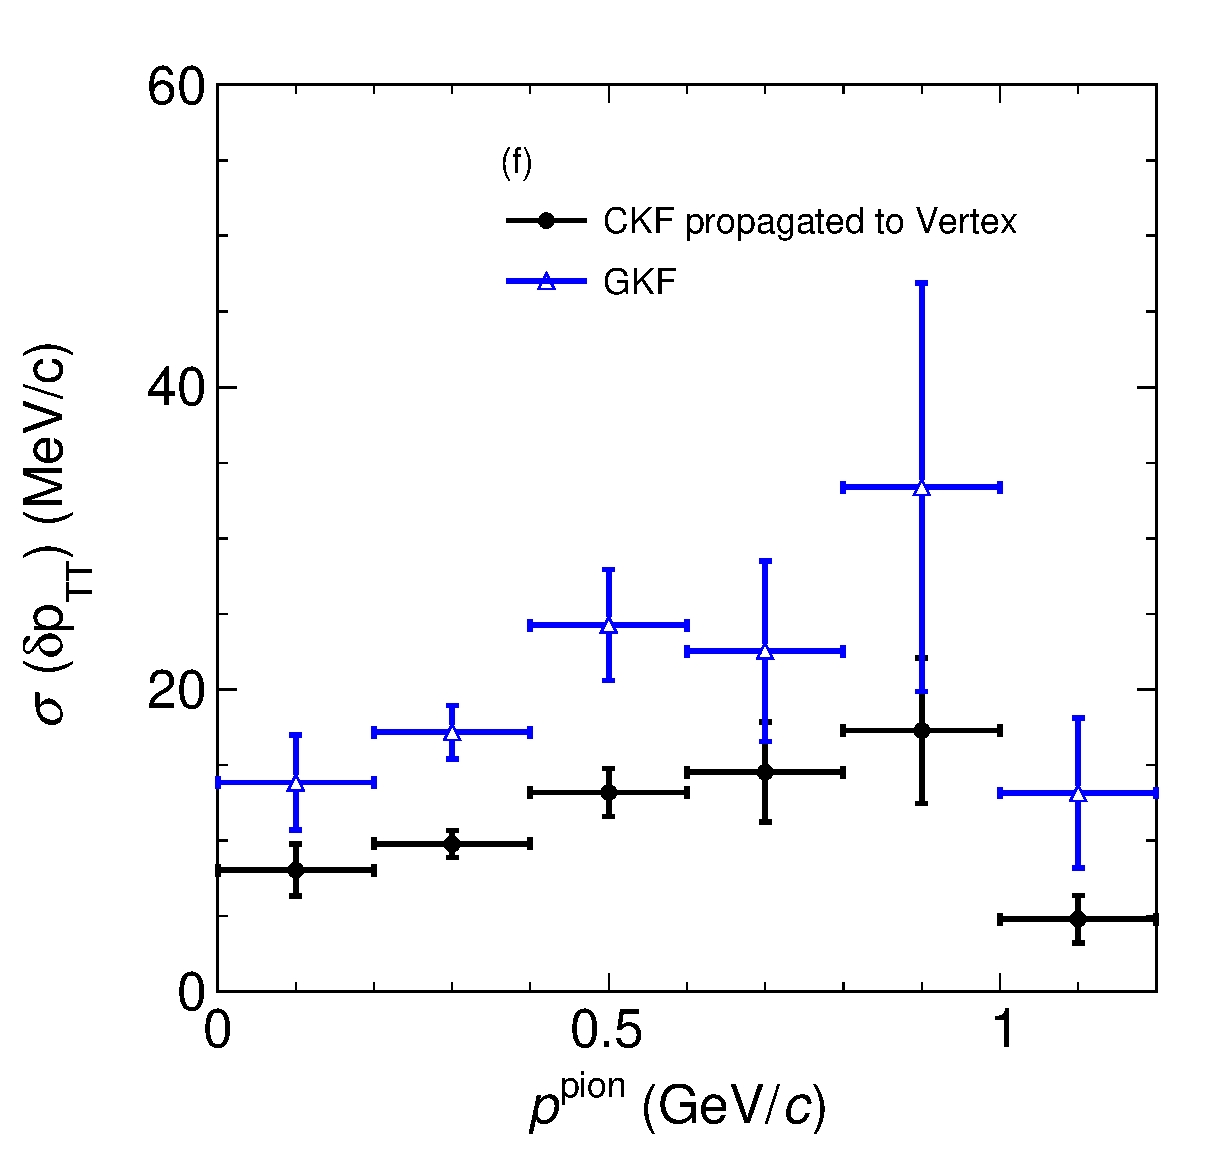
\includegraphics[width=\textwidth]{figures/ch6-TKI/2D/deltapTTVSp211.eps}
         \caption{}
         \label{fig:deltapTTVSp211.eps}
     \end{subfigure}

              \begin{subfigure}[b]{0.32\textwidth}
         \centering
         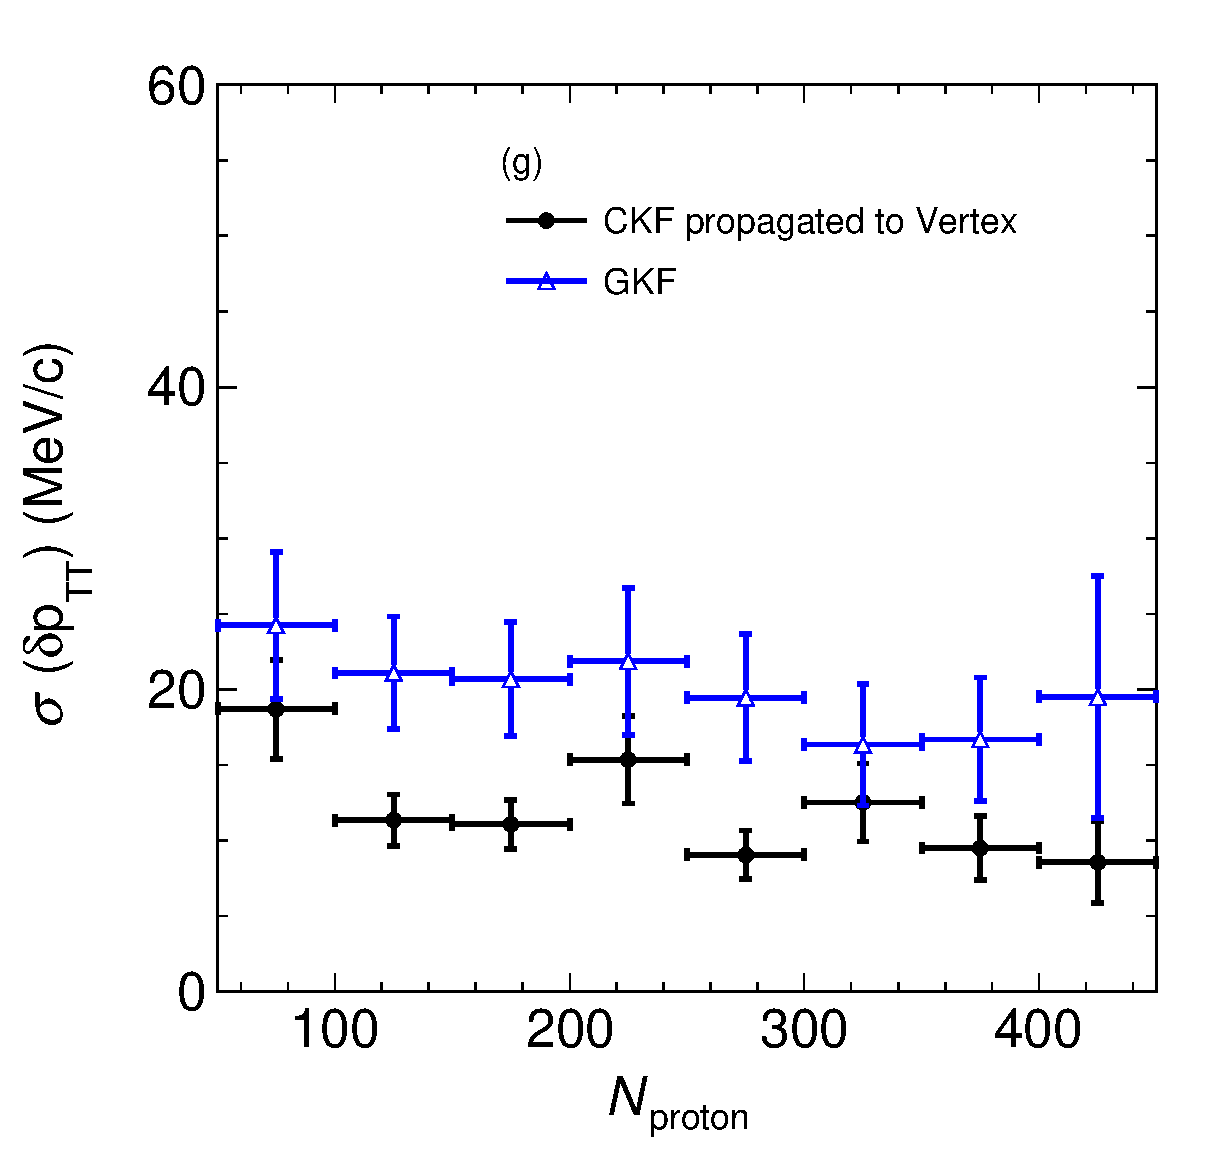
\includegraphics[width=\textwidth]{figures/ch6-TKI/2D/deltapTTVSN2212.eps}
         \caption{}
         \label{fig:deltapTTVSN2212}
     \end{subfigure}
     \begin{subfigure}[b]{0.32\textwidth}
         \centering
         \includegraphics[width=\textwidth]{figures/ch6-TKI/2D/deltapTTVSlArmMC2212.eps}
         \caption{}
        \label{fig:deltapTTVSlArmMC2212.eps}
     \end{subfigure}
     \begin{subfigure}[b]{0.32\textwidth}
         \centering
         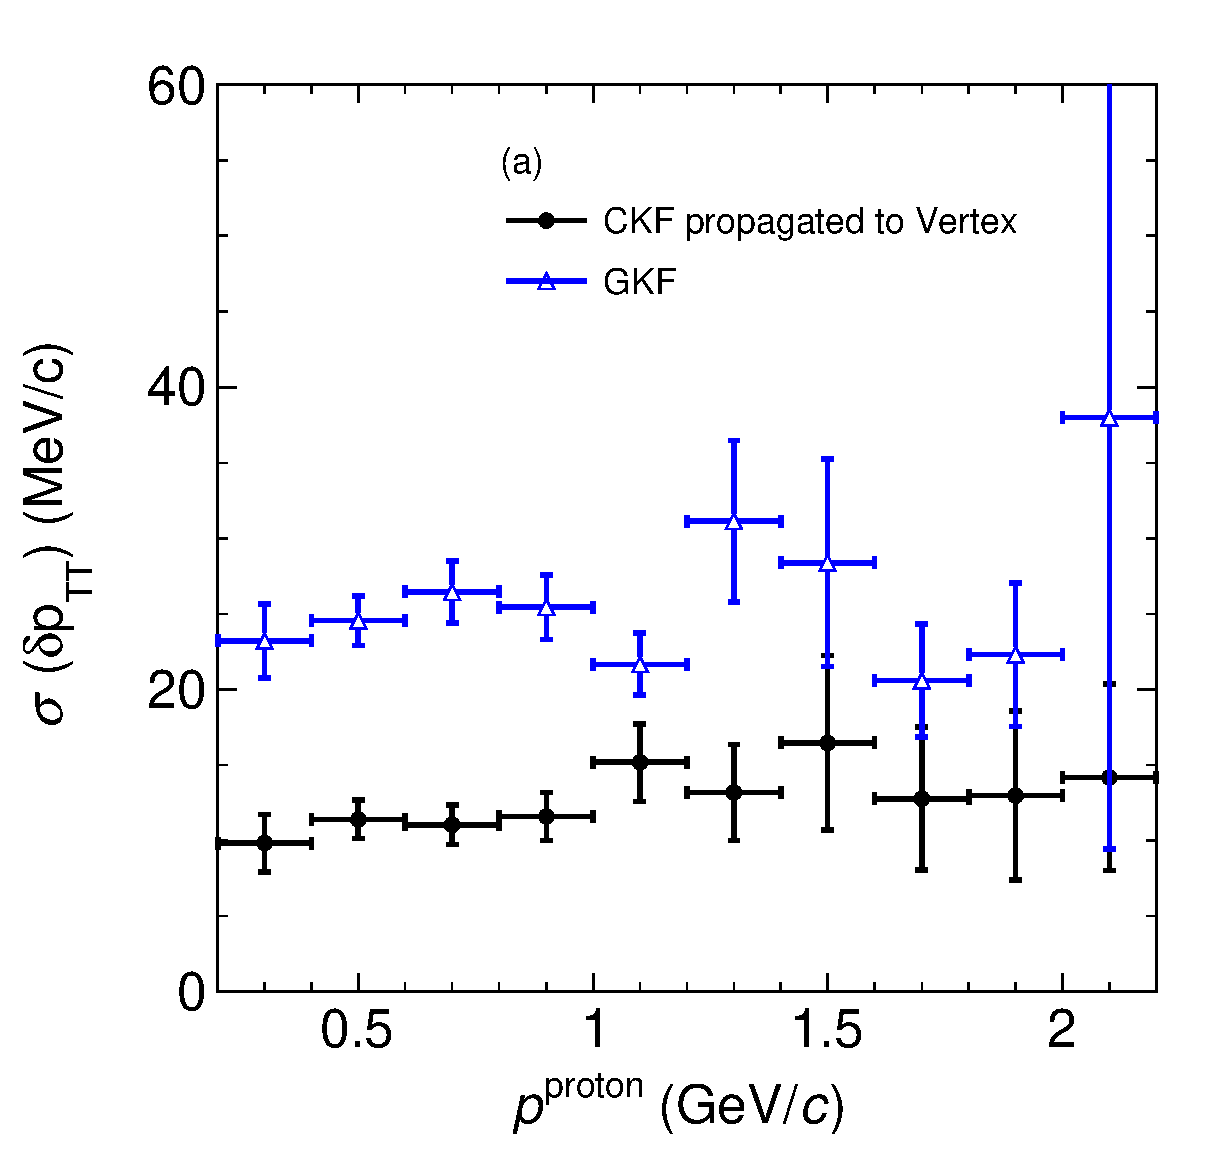
\includegraphics[width=\textwidth]{figures/ch6-TKI/2D/deltapTTVSp2212.eps}
         \caption{}
         \label{fig:deltapTTVSp2212.eps}
     \end{subfigure}
        \caption{Dependency of the $\delta p_\texttt{TT}$ Cauchy spread Hydrogen resolution as a function of number of points $N$, lever arm $L_\text{Arm}$ and true initial momentum $p$ for the three particle types in increasing order of mass from top to bottom: muons, pions and protons. In blue we show the results obtained with the \texttt{\texttt{GKF}}, while in black we show the results for the \texttt{\texttt{CKF}} propagated to the reconstructed vertex.} \label{fig:dpTTVSpart}
\end{figure}

Using the $\delta p_\text{TT}$ resolution found for the \text{\texttt{CKF}} algorithm after the reconstructed vertex propagation (see Fig. \ref{fig:dpTT_ALICEStRecoGArReco}), which is $\sigma(\delta p_\text{TT})=(12\pm1)\ \text{MeV}/c$, we can impose the cuts $|\delta p_\text{TT}|\leq n\sigma$. We identify the signal as the Hydrogen target sample and the background as either the Carbon target sample, the Argon target sample or the combination of both. We define the cut efficiency $\epsilon_{\delta p_\text{TT}}$ as the ratio between signal and background events passing the cut and the total number of events:
\begin{equation}
    \epsilon_{\delta p_\text{TT}} = \frac{N_\text{sig}^\text{pass}+N_\text{bkg}^\text{pass}}{N_\text{sig}^\text{tot}+N_\text{bkg}^\text{tot}}
\end{equation}
We can also define the purity $\rho_{\delta p_\text{TT}}$ as the ratio between the number of signal events that passed the cut and the number of total events that passed the cut:
\begin{equation}
    \rho_{\delta p_\text{TT}} = \frac{N_\text{sig}^\text{pass}}{N_\text{sig}^\text{pass}+N_\text{bkg}^\text{pass}}
\end{equation}
We calculated the efficiency and purity for the $|\delta p_\text{TT}|\leq n\sigma$ cut for $n=1,2,3$ considering as the background the Carbon and Argon events both separately and in total. The results are summarized in Tab. \ref{tab:dpTT_eff+pur}. As previously discussed, using ND-GAr's nominal gas mixture, the Argon background completely dominates and makes the application of the technique not practical. If we just consider the Carbon background however, the results are much more encouraging, showing a purity of at a $1\sigma$ cut of $\rho_{\delta p_\text{TT}}=(81\pm6)\%$. It's clear that in order to reap the benefits of the $\delta p_\text{TT}$ technique in ND-GAr, other gas mixtures should be considered. 



\begin{table}
    \centering
    \begin{tabular}{||c|c|c|c|c|c|c||}
         \hline
          $(\%)$&  $\rho \ (\ 1\sigma)$&  $\rho \ (\ 2\sigma)$&  $\rho \ (\ 3\sigma)$&  $\epsilon \ (\ 1\sigma)$&  $\epsilon \ (\ 2\sigma)$&  $\rho \ (\ 2\sigma)$\\
         \hline \hline
         C &  $81\pm6$&  $76\pm4$ & $69\pm4$  &  $19\pm1$& $26\pm1$ &$33\pm1$ \\
         \hline
         Ar &  $17.6\pm0.9$& $13.0\pm0.6$ & $10.2\pm0.4$ & $5.7\pm0.1$ & $10.5\pm0.2$ & $15.0\pm0.2$\\
         \hline
         Ar+C& $16.9\pm0.9$ & $12.5\pm0.6$ & $9.7\pm0.4$ & $5.7\pm0.1$  & $10.5\pm0.2$ & $15.0\pm0.2$\\
         \hline
    \end{tabular}
    \caption{Efficiency $\epsilon_{\delta p_\text{TT}}$ and purity $\rho_{\delta p_\text{TT}}$ for the $|\delta p_\text{TT}|\leq n\sigma$ cut for $n=1,2,3$ for a signal of Hydrogen events, considering as the background the Carbon and Argon events both separately and in total. The $\sigma$ used is the Cauchy spread estimated for the \texttt{CKF} algorithm after vertex propagation.}
    \label{tab:dpTT_eff+pur}
\end{table}



